\documentclass[12pt,a4paper,notitlepage]{article}
\usepackage[margin=1.5cm]{geometry}
\usepackage{cite}
\usepackage[font=small,labelfont=bf]{caption}
\usepackage{graphicx}
\usepackage{placeins}
\usepackage{booktabs}
\usepackage{xspace}
\usepackage{longtable}
%\usepackage{arev}
\usepackage{titlesec}
\titleformat{\section}{\large\bfseries}{\thesection}{1em}{}
\titleformat{\subsection}{\normalsize\bfseries}{\thesubsection}{1em}{}
\usepackage{url}
\usepackage{hyperref}
\hypersetup{
  pdftitle={Report},    % title
  pdfauthor={Vittore F. Scolari},     % author
  pdfsubject={Brownian dynamic simulations},   % subject of the document
  colorlinks=false,       % false: boxed links; true: colored links
  pdfborder={0 0 0}
}
\usepackage[toc,page]{appendix}
\usepackage{amsmath}
\usepackage{amsfonts}
\usepackage{mathrsfs}
\usepackage{mathtools}

\newcommand{\fis}{\emph{Fis}\xspace}
\newcommand{\crp}{\emph{CRP}\xspace}
\newcommand{\hns}{\emph{H-NS}\xspace}
\newcommand{\camp}{\emph{cAMP}\xspace}
\newcommand{\ecoli}{\emph{E. coli}\xspace}
\newcommand{\ve}[1]{\mathbf{#1}}
\newcommand{\nm}{\mathrm{nm}}
\newcommand{\dna}{\emph{DNA}\xspace}
\newcommand{\rna}{\emph{RNA}\xspace}
\newcommand{\nap}{\emph{NAP}\xspace}
\newcommand{\naps}{\emph{NAPs}\xspace}
\DeclareMathOperator{\median}{median}
\newcommand{\blankpage}{\newpage\thispagestyle{empty}\mbox{}\newpage}

\begin{document}
\title{Simulations of collapsed polymers as a simple model of
  bacterial nucleoids}
\author{Vittore F. Scolari and Marco Cosentino Lagomarsino}
\maketitle
We aim at using computer simulations in order to test models which can
 predict the experimental measurements
\cite{Lieberman2009, Weber2010, Barbieri2012}
that show insight about the physical organization of the \dna polymer and
the interaction with Nucleoid associated proteins (\naps).

The \dna in \ecoli is a polymer with arc-length of $1.57$mm and
diameter of $2.37$nm which gets continuosly replicated over a period
of $40$ minutes. The Nucleoid is a protein-\dna complex where the
active processes which are related to the \dna functionality such as
transcription and replication happen inside the bacterial cell. Thus
the nucleoid is made of \dna, \rna, and various functional proteins such
as transcriptiona factors, nucloid associated proteins, \rna and \dna
polymerases which bind, associate and interact each other in order to
make dynamic and static structures. 

It is known that the nucleoid is collapsed in a volume which is
comparable to $1/6$ of the cell\cite{}, this property not only makes
the polymer much smaller than the volume between the cell walls but
also it results in a
%% cambiare parola
stronger viscoelastic behaviour\cite{Wiggins2010}. Two possible mechanism
have been proposed for the collapse of the
nucloid: confinement due to the cell walls\cite{} and depletion due to
the interaction with the cytoplasm\cite{}. The first hypotesis is in
contradiction with the fact that the nucleoid occupies only a small
region of the bacterial cell, while the second is in agreement with
recent experiments which \cite{Pelletier2012} have shown
that purified nucleoids can collapses due to the depletion with a
crowding agent ({\it PEG}); the concentration of proteins in the
cytoplasm is comparable to the concentration of {\it PEG} which
collapse the \dna in purified nucleoid just at the transition between
coiled and collapsed state.

An important role in the \dna organization in the nucleoid is played
by the \naps, proteins which bind and structure the \dna. The role of
\naps is still a research subject and it has been shown that most of
them have also a fundamental role in gene expression regulation as
hubs of the transctiptional network of \ecoli. Between all of them
\hns is particularly interesting because it make crosslinks between
different segments of the \dna bringing part of the distant part of
the chromosome in the genome close together in space and also because
it can oligomerize thus making complexes which bind strongly to
\dna. Recent experiments have shown that \hns is the only \nap which
makes between two and four foci, which are globules where the protein
with the bound \dna aggregates, into living cells.

In this work we will investigate a model for the \dna in the nucleoid
as a polymer which cooks two ingredients:
a weak glue that describe the depletion of the molecular crowding to
the nucleoid and a strong localized interaction which describes the
binding of \hns to the binding sites. We aim at exploring the
different configuration possibilities of the nucleoid following the
varying of the those different kind of interctions.

\section{The model}
\label{sec:themodel}

The \dna is a polymer with Khun length of $\sim 105 \mathrm{nm} (308
\mathrm{bp})$ and diameter of $2.37 \mathrm{nm}$. In \ecoli \dna is a
single circular polymer of length $\sim 1.577 \mathrm{mm} (4639
\mathrm{kbp})$.

We simulate the \dna polymer as a bead spring model. In our model the
polymer segments are represented by beads in three dimensional
space. The number of beads which we use to represent the polymer is
arbitrary, we call this parameter $N$. We define four fundamental
forces on the beads in order to obtain a macroscopical description
which reproduces the phenomena we want to investigate about the
nucleoid. Each of these forces define a term in the interaction
energy.
\begin{enumerate}
\item
  {\bf The chain links force}: in the \dna molecule monomers are
  covalently bounded together to form a polymeric chain. In our model
  we represent this connectivity by a link network which connect
  the beads which represent adjacent segments of the chain. The
  distance in three dimensional space between two bead which are
  linked correspond to the length of the link.
%   The energy term can be described by:
% \begin{equation}
%   E_{link} = \lim_{a \to \infty} \left[ a \sum_{i,j = 1}^N A_{ij} \theta
%   (\lambda - |\vec r_i - \vec r_j |) \right]
% \end{equation}
%   Where $A_{ij}$ is the adjacence matrix of the connectivity network and
%   $\theta()$ is the step function.
  We assign an infinite energy to every configuration which carry a
  link longer than a characteristic length $\lambda$.
\item
  {\bf The hard core repulsion}: the \dna molecule self-interact
  through electromagnetic forces. In ionic solutions this correspond
  to a short ranged repulsion between different part of the
  polymer. Due to this force different segment of \dna does not overlap
  with each other. In our model we set a minimum distance $\sigma$
  between every bead and we assign an infinite energy to all
  configurations which carry two beads at a smaller distance.
\item
  {\bf Cytoplasm protein crowding}: the concentration of proteins in the
  cytoplasm is enough to collapse the \dna into a globular state
  \cite{Pelletier2012}. The depletion of the macromolecules in the
  cytoplasm due to the presence of the long \dna macromolecule results
  in an effective attraction between couples of \dna double Helix
  segments, the range of this force is comparable to the diameter of a
  typical crowding protein. In our model we represent this force as a
  weak attractive glue between every bead. The configuration energy will
  be decremented by $\epsilon_u$ for every couple of beads which are
  at a distance smaller than a the characteristic length of attraction
  $\alpha$, this gives more stability to the configuration.
\item
  {\bf \dna binding proteins}: \hns makes crosslinks between
  different segments of the \dna, it can oligomerize thus it makes
  strong bounded complexes. This mechanism mediates for an effective
  attraction between the binding sites of \hns. In our model we
  represent this force as a strong attractive localized interaction
  between a selected set of beads which represent the ones which carry
  a \hns binding sites. The configuration energy will be decremented
  by $\epsilon_l$ ($\epsilon_l > \epsilon_u$) for every couple of
  binding site carrying beads which are at a distance smaller than
  the characteristic length  of attraction $\alpha$.
\end{enumerate}

The interaction potential can be described by a function of  
the distance between interacting pairs of beads $U(r)$, which is
reported in Fig. \ref{fig:potential}.

\begin{figure}[h!]
\centering
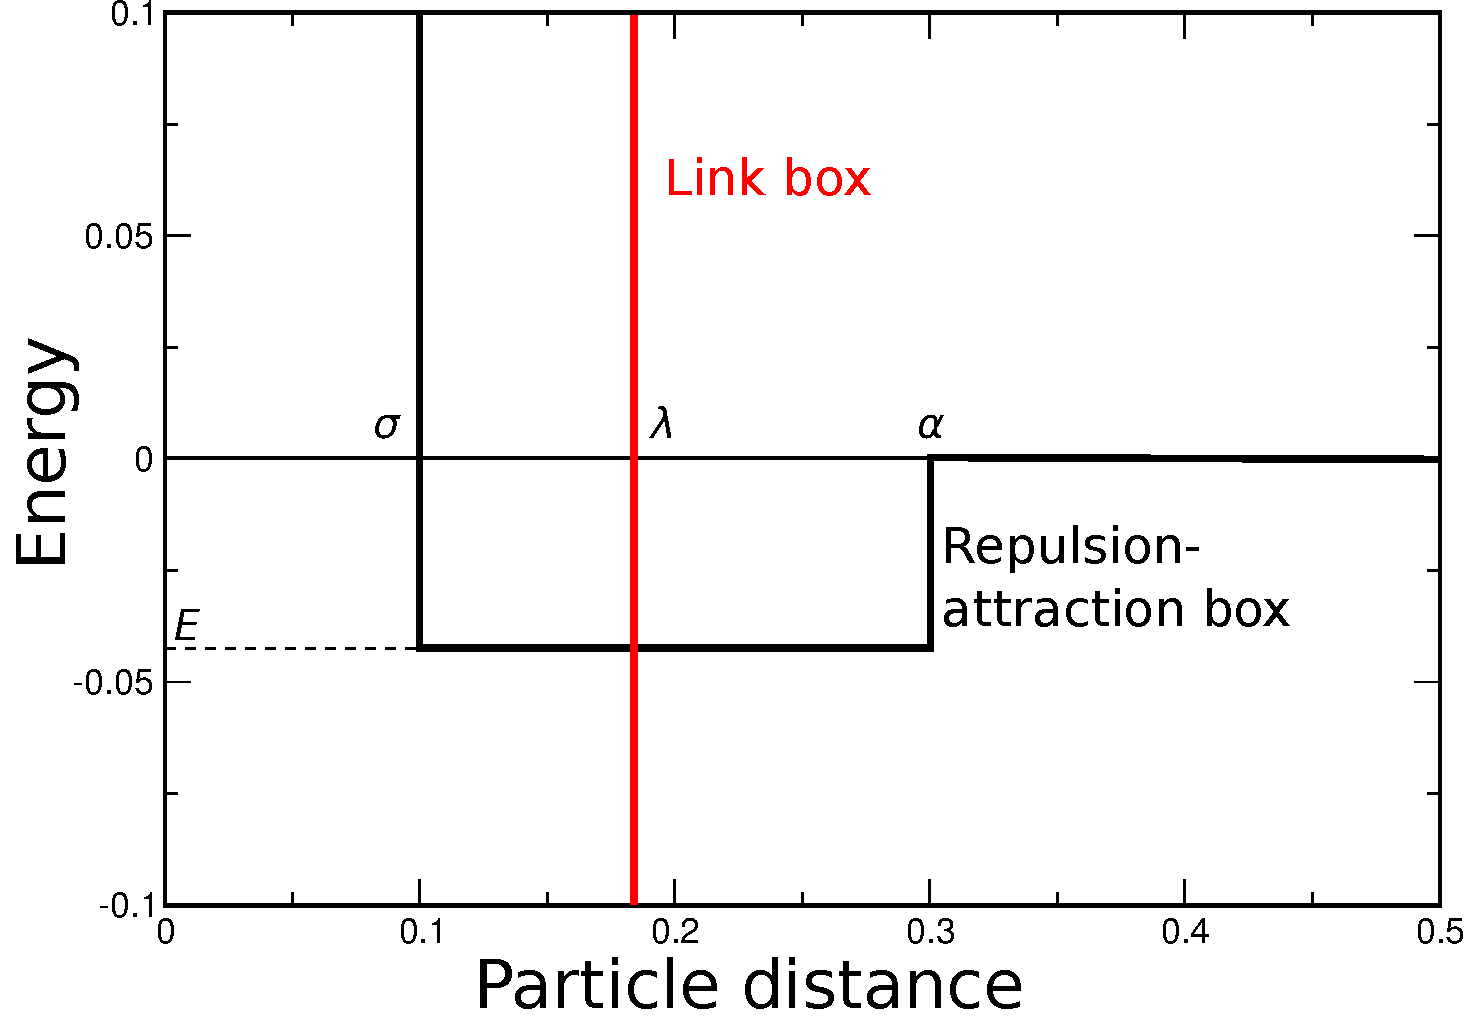
\includegraphics[width=10cm]{potential}\\
\caption{The interaction potential: The link potential (red
  line) imposes beads which are connected in the 
  chain to be close to each other;
  % in reality \dna is quite a stiff polymer
  % which would show a very different kind of potential but which will
  % converge to Gaussian statistics at larger scale as our defined
  % potential does. This model is thus an effective model valid for a
  % coarse grain description of the \dna chain. Estimation of the scale of
  % validity of the quantitative predictions of the model is to be done if
  % possible.
  % 
  the interaction potential (black line) represent the energy in
  function of the distance between different interactiong beads $U(r)$
  which is the sum of an hard-core repulsion and an attraction box.
  % The repulsion is due to electrostatic
  % interactions which are of short range by nature (Debye screening
  % length). The attraction box can be due to multiple factors: it can be
  % due to the effect of depletion between the \dna molecule and the
  % cytoplasm \cite{Odijk1998}, due to the effect of electrostatic
  % interaction of nonspecific divalent ions measured in vitro by
  % \cite{Qiu2007} or due to the presence of nucleoid associated proteins
  % (\naps) like \fis, \crp and \hns which act as \dna binders and make
  % cross-links between different segments of the chain \cite{Dorman2004};
  % in a later version of the model we will place those kind of interaction
  % not uniformly along the chain.}
}
\label{fig:potential}
\end{figure}

In this model we disregard the possible liquid crystalline ordering of
interacting \dna chains \cite{Nakata2007}.

\section{Monte Carlo algorithm}
We use an off lattice Monte Carlo algorithm with Metropolis rejection
rule in order to simulate the polymer configuration in the Gibbs
ensamble. 
% This Monte Carlo simulation explores the phase space of the
% selfavoiding polimer and permit a measure of the mean values of
% equilibrium observables such as the extension and the relative
% position of the monomers in the model. This approach gives us the
% possibility to quickly extend the model by adding discrete and
% complicate kind of interactions (like the effect of \naps) and test the
% effect of those interactions on the observations.  This approach
% does not permit us to make dynamical measurements of
% out-of-equilibirium properties of the model because the Monte Carlo
% dynamic does not necessarily correspond to the pysical dinamics of the
% self avoiding polymer; those properties can be explored using Brownian
% dynamics simulations.
In every step
the algorithm moves a random bead of the chain by a vector
chosen with a uniform spherical distribution of radius $\Delta r$,
then acceptance rules are applyed according to the defined
fundamental forces. A resume of the acceptance rules is give in
Fig. \ref{fig:montecarlo}.
\begin{figure}[h!]
\centering
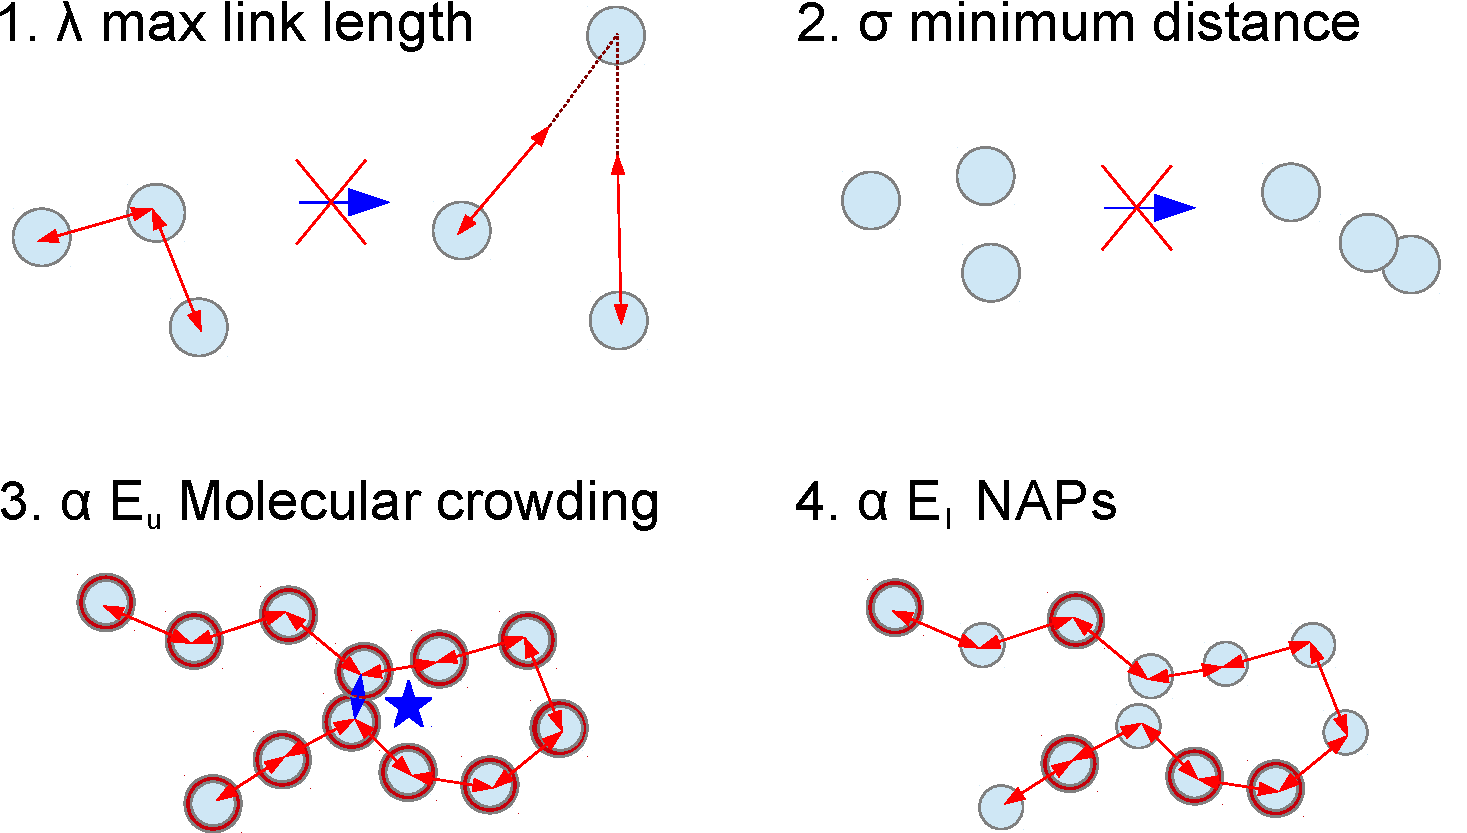
\includegraphics[width=12cm]{montecarlo}\\
\captionsetup{singlelinecheck=off}
\caption[Acceptance rules of the montecarlo algorithm.]{
  Acceptance rules of the montecarlo algorithm.\\
  \begin{enumerate}
  \item
    Maximum link length: every new configuration which have a link
    longer than $\lambda$ is rejected.
  \item
    Hard core repulsion: every new configuration in which there is a
    couple of beads with distance smaller than $\sigma$ is rejected.
  \item
    Uniform attraction: for every new configuration, the difference in
    energy due to the molecular crowding is evaluated. The
    Metropolis acceptance rule is applied in order to reject low
    probability configurations.
  \item
    Localized attraction: for every new configuration, the difference in
    energy due to the localized binding-protein mediated attraction is
    evaluated. The Metropolis acceptance rule is applied in order to
    reject low probability configurations.
  \end{enumerate}
}
\label{fig:montecarlo}
\end{figure}

Our algorithm was inspired by a work on the
behaviour of polymers under confinement\cite{Cacciuto2006a}.

By considering only the energy interactions, it is not possible to
guarantee topological invariance of ring polymers.
 % as long as $\lambda > (\sqrt{2} \sigma - \Delta r)$
A supplementary topological interaction acceptance rule have been
implemented in order to overcome this limitation.

\subsection{Topological interaction}
In order to prevent the dynamic to break topological barriers, the
simulation need to avoid any monomer movement which would cross two
links of the polymer. We do so by testing the interseption between
each link of the polymer seen as segment in three dimensional space
and the two triangles spanned by the movement of the links connected
to the monomer which is to be moved (see fig.\ref{fig:triangolo}).
\begin{figure}[h!]
\centering
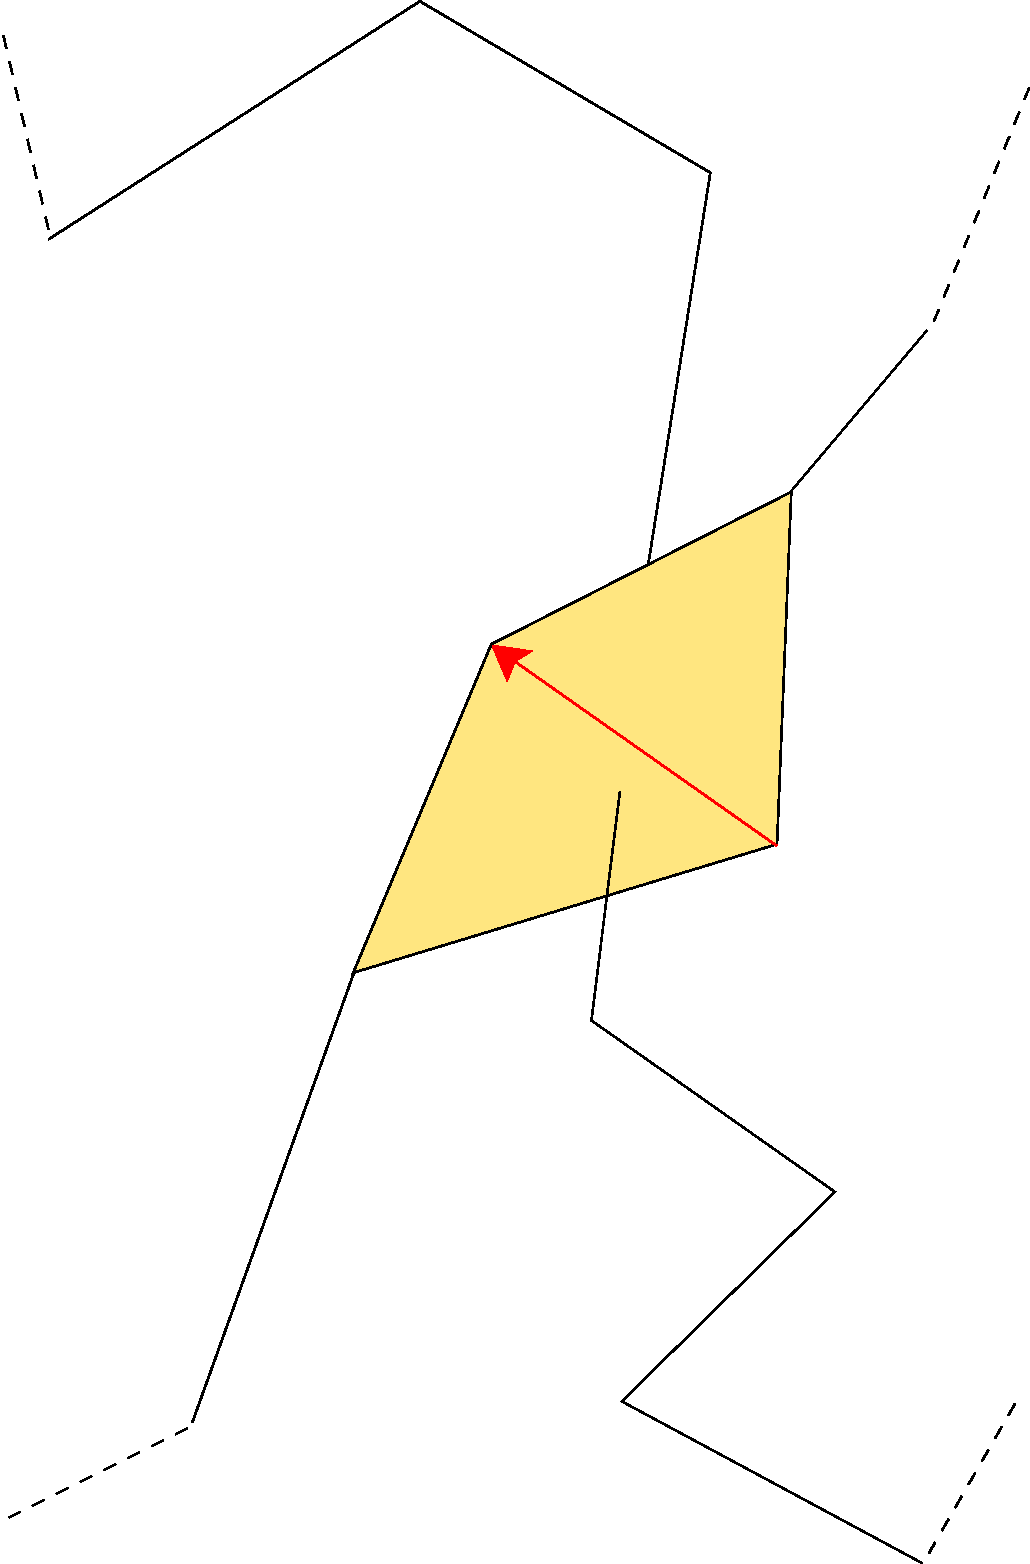
\includegraphics[angle=90,width=6cm]{triangolo}\\
\caption{Rejected topological move, the yellow area represent the
  two triangles spanned by a MC move (red arrow).}
\label{fig:triangolo}
\end{figure}
We test this interseption using common ray-tracing algorithms
\cite{Moeller1997} and in the positive case we reject the 
move.
% Note: of course here a lot of work can be done from measuring
% knot polynomial in the simulation (polygonal chains, an article in
% mathematics can be written just on that) to connect this kind of local
% interaction to conservation of topological quantities, to see the
% effect of this kind of interaction on the dynamics of the polymer.

\FloatBarrier
\section{Thermodinamic of the single polymer}

\label{par:parameters}
Our approach is to simulate the \dna in the nucleoid as a bead spring
model. In this model the number of beads $N$ is arbitrary and fixes
the amount of details we take into account: by taking a
smaller number we save computational resources but we are in fact
re-summing the degree of freedom of the system and discarding all the
microscopical details for contour lengths less then $2L/N$ (where $L$
is the length of the polymer); on the other end it seems reasonable to
discard those details since a gene in \ecoli is normally $1
\mathrm{kb}$ long and we don't really have enough information to go at
resolution lower than that.

We want to keep the freedom of choosing the appropriate $N$. The other
parameters ($\lambda, \sigma, \alpha, \epsilon_u,$ and $\epsilon_l$)
need to be choosen as a function of $N$ in order to keep the 
results consistents at different values. The parameters need to be set
and compared to biophysical quantities of the nucleoid so we elaborated
a {\it protocol} explained in the following sections in order to be
able to set them.

\subsection{Square distance as a function of arc-length}
A statistical configuration of a polymer in our model is completely
described by $N$ vectors $\{ \vec r_i \}_{i \in 1 .. N}$ which
identify for each bead its position. Due to the translational simmetry
for the center of mass, the rotational symmetry in three dimensional
space, and the translational simmetry on the chain backbone (in
the circular polymer case) it is more convenient to take the mean
square distance $R$ between beads as a function of their arc-length
distance $s$, $\langle R^2 (s) \rangle$, as the main observable we
measure in our simulations.

Through $\langle R^2 (s) \rangle$ it is possible to measure the size
of the polymer and also to extimate the probability of loop formation
as a function of the arc-length; this observable is thus connected to
the results of the biological experiments of Fluorescence in situ
hybridization ({\it FISH}) and Chromosome conformation capture
({\it Hi-C}).

\subsection{Scaling of the link length parameter $\lambda$, the ideal polymer}

In the case where we neglect all the interaction forces between beads
(the hard core repulsion, the molecular crowding and the localized 
interactions) but we keep a linear polymer link connectivity we obtain
a model which describes {\it the ideal polymer}. In
absence of other energetic or topological constraints, the separation
in space for two beads in an ideal polymer can be calculated easily in
the following way:
\begin{equation}
  \vec R(s) = \vec b_1 + \vec b_2 + \dots + \vec b_s = \sum_{i=1}^s
  \vec b_i \qquad \mathrm{where} \qquad \vec b_i = \vec r_{i+1} - 
  \vec r_i.
\label{eq:idealbees}
\end{equation}
The square distance as a function of the arc-distance is:
\begin{equation}
  \langle  R^2(s) \rangle = \langle \vec R(s) \cdot \vec R(s) \rangle
  = \langle \sum_{i=1}^s \vec b_i \cdot \sum_{j=1}^s \vec b_j \rangle
  = \langle | \vec b_i || \vec b_j | \cos \theta_{ij} \rangle
  = \langle b^2 \rangle s.
\label{eq:idealettoe}
\end{equation}
and in our specific case, where $\vec b_i$ are random vector in the
sphere of radius $\lambda$:
\begin{equation}
  \langle b^2 \rangle = \frac{3}{5}\lambda^2, \qquad \mathrm{and}
  \qquad \langle  R^2(s) \rangle = \frac{3}{5} \lambda^2 s.
  \label{eq:elldef}
\end{equation}

This latter formula show that for the ideal polymer the scaling of the
square distance as a function of the arc-length is predictable for our
model.
We can use this prediction to define a practical unit of length $l_0$
by setting, for every $N$, the mean end-to-end
distance in units of $l_0$ to unity:
\begin{equation}
  \langle R^2(N) \rangle / {l_0}^2 \equiv 1;
\label{eq:lzerodef}
\end{equation}
which implies the {\it first rule of parameter normalization}:
\begin{equation}
\hat \lambda^2 \equiv \left( \frac{5}{3}\frac{1}{N} \right).
\label{eq:lambdadef}
\end{equation}
This latter formula fixes the scaling of the link length $\lambda$ in
function of the arbitrary parameter $N$. In this and in the following
formulae we use an hat (as in $\hat \lambda$) on top of length-type
variables in order to express their numerical value in units of
$l_0$. In our model the link length $\hat \lambda$ does not depend on
any other parameters than $N$.

\begin{figure}[h!]
\centering
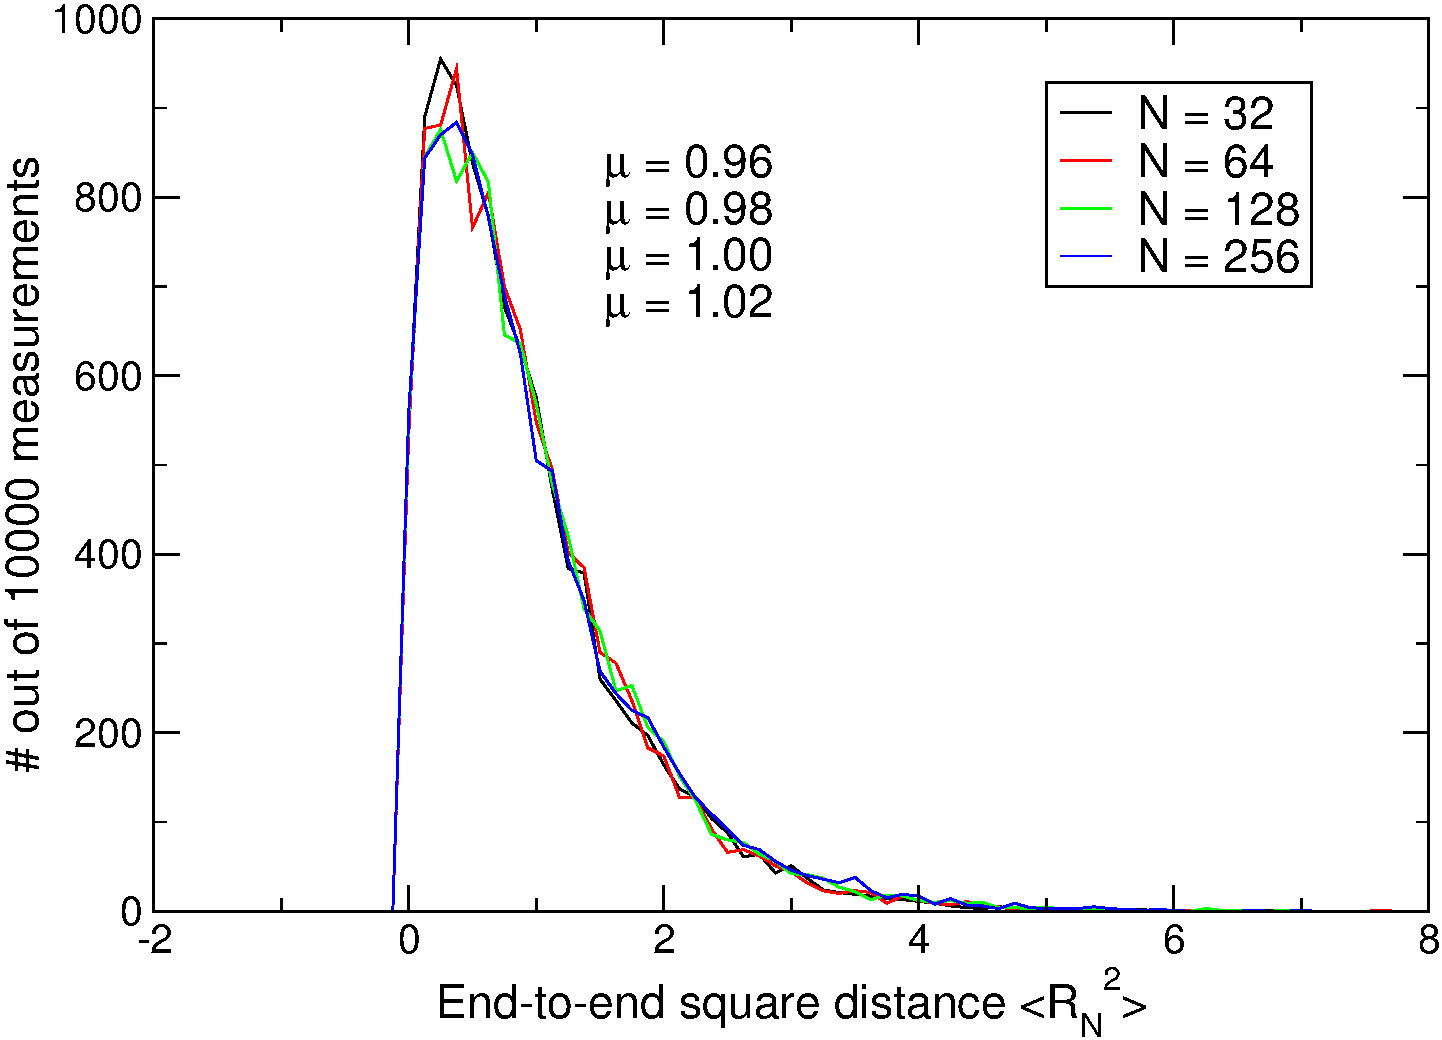
\includegraphics[width=9cm]{RW_renorm}\\
\caption{$\langle \hat R^2(N) \rangle$ with $N = 32, 64, 128, 256$ for
  the ideal polymer. The distribution is the same  regarding the value
  of the resolution $N$ after proper normalization of parameter
  $\lambda$ using formula \ref{eq:lambdadef}. The unit length is equal
  to $l_0$ thus the distibutions have unit mean values.}
\label{fig:RWrenorm}
\end{figure}

\FloatBarrier
\subsection{Free energy of the ideal polymer}
The Helmholtz free energy $F(\vec r)$ associated with all chain
conformation starting from an origin $(\vec r = 0)$ and ending at the
point $\vec r$ is simply related to the number of distinct polymers
with $N$ beads $\mathbb{Z}_N(\vec r)$ going from $(0)$ to $(\vec r)$:
\begin{equation}
  F(\vec r) = - k_b T \ln \left[ \mathbb{Z}_N( \vec r ) \right].
\label{eq:entropy}
\end{equation}

The probability distribution $\rho$ of $\vec r$ defined by 
\begin{equation}
  p_N(\vec r) = \frac{\mathbb{Z}_N( \vec r )}
  { \int_r \mathbb{Z}_N( \vec r )},
\end{equation}
for the ideal polymer is given by the convolution of the distributions
of consecutive $\vec b_i$ as defined in Eq. \ref{eq:idealbees}.
For $s \gg 1$ due to the central limit theorem we can extimate that
\begin{equation}
  p_N \left( \vec r \right) =
  \left ( \frac{5 \pi}{2 \lambda^2 N} \right)^{3/2}  \exp \left(
    - \frac{5}{2} \frac{\vec r^2}{\lambda^2 N} \right) =
  \left ( \frac{3 \pi}{2 {l_0}^2} \right)^{3/2}  \exp \left(
    - \frac{3}{2} \frac{\vec r^2}{{l_0}^2} \right).
\label{eq:probideal}
\end{equation}

The above end-to-end distribution combined with Eq. \ref{eq:entropy}
gives an important formula for the {\it entropy of the ideal polymer}
at fixed elongation:
\begin{equation}
  F_{ideal}(\vec r) = F(0) + \frac{3}{2 {l_0}^2} k_b T 
  \langle \vec r^2 \rangle,
\label{sideal}
\end{equation}

By deriving we can write the equation of state for the tension in
function of elongation for the ideal polymer:
\begin{equation}
  \tau_j = - \frac{\partial F}{\partial r_j} = - 3 \frac{k_b T}{l_0}
  \cdot \frac{r_j}{l_0}
\end{equation}
which resembles the spring equation. This equation is valid only for
the cases in which the hard core repulsion and the attractive
interactions are negligible. It has been tested in
microrehological experiments by measuring the mechanical response of
\dna or other polymers attached to dielectric beads under deformation
applyed using optical traps and it has been found as a good first
order approximation. Under strong stretching ($\tau_j \gg k_b T / l_0$)
the Gaussian distribution (eq. \ref{eq:probideal}) is not a valid
model for the polymer due to the finite exensibility of the chain and
a alternative potentials should be used instead (cite Siggia).

This equation have been also recently used as a null model (cite
Wiggins) for the bacterial necleoid, it's derivation is obtained by
neglecting interactions of the polymer with himself and for this
reason the results of the experiment didn't agree with this simple
theory. Although the effect of finite extensibility can be important
in the microscopic DNA processes we consider this effect not relevant
for the eqauilibrium state of the Nucleoid.

We can check the consistency of the free energy and the equation of state
by calculating the extensibility, which should be equal to the fluctuations
of $r_j$:
\begin{equation}
  \langle \vec r^2 \rangle = k_b T \sum_j \frac{\partial r_j}{\partial
    \tau_j}  = {l_0}^2.
\end{equation}

\subsection{Coil-globule transition}

In the following three paragraph we try to understand the behavior of
our model by describing the configurations that the polymer assumes in
presence of the hard core repulsion (electromagnetic) and the uniform
attraction (molecular crowding of the cytoplasm). Note that
we still neglect {\it only} the localized interaction (crosslinking
proteins).

In presence of repulsive and attractive interactions some aspect of
the behaviour of the polymer are well known and intuitive. If the
interactions are repulsive only ($\epsilon_u = 0$) the polymer is in the coil
phase: the volume increase, and the scaling of $R^2(s)$ differ from
the linear dependence on $s$ (see Eq. \ref{eq:elldef}) in the ideal
polymer case. If, in the opposite case, we take configurations at very
strong attraction energy ($\epsilon_u \to \infty$) the effect of attraction
overwhelm the repusion due to hard core interactions and the polymer
collapse in a globular compact state. Between the two extreme
conditions the polymer undergoes a phase transition (represented in
Fig. \ref{fig:collapse}).

In order to qualitatively describe the transition from coil to
globular state we can introduce the effect of two-beads
interactions in the free energy as a virial coefficient expansion:
\begin{equation}
  F_{coil} = F_{ideal} + k_bT v \rho^2 V
\end{equation}
where $\rho \equiv N/V$ is the number density of the polymer
beads and $v$ is the effective volume of interaction of a bead of the
polymer to other beads. This procedure will lead to what is known as
the Flory-Huggins theory of the interacting polymer.

The above free energy can be rewritten explicitly in volume and number
of beads by setting with a mean field approach $V$ as a function of the
size of the fluctuations of the end-to-end distance:
\begin{equation}
  F_{coil} = F(0) + \frac{5}{2} \frac{k_b T}{\lambda^2 N}V^{2/3}
  + k_b T N \left(
  \frac{N - 1}{2} \frac{v}{V} \right) \qquad \mathrm{with} \qquad
    \langle \hat R^2 \rangle \approx \hat V^{2/3};
\label{eq:floryent}
\end{equation}

The calculation of the effective volume of interaction $v$ shows the
different behaviour of the system, with respect to the ideal polymer
case, as a function of the ratio between the interaction energy and the
temperature $\epsilon_u/k_b T$. Since the interaction energy $U_u(r)$
(represented in Fig. \ref{fig:potential}) is a function of only
the mutual distance between two beads in the model, we can obtain the
effective volume of interaction $v$ by integrating the Mayer
$f$-function defined as $f(r) = \exp [-U_u(r)/k_b T] - 1$ over the
distance between two beads:
\begin{equation}
  v \equiv - 4 \pi \int_0^{\infty} f(r) r^2 dr \approx
  4 \pi \int_0^{\sigma}r^2 dr -
  \frac{4 \pi}{k_bT} \int_{\sigma}^{\alpha} \epsilon_u r^2 dr \approx
  b - \frac{a}{k_b T},
\label{eq:effvol1}
\end{equation}
where
\begin{equation}
  b = \frac{4}{3} \pi \sigma^3 \qquad \mathrm{and} \qquad
  a = \frac{4}{3} \pi \epsilon_u (\alpha^3 - \sigma^3).
\label{eq:effvol2}
\end{equation}

From this formulation it is possible to extract the critical energy of the
coil-globule transition. A null effective volume is obtained for 
$a = (k_b T) b$:
\begin{equation}
  \hat \epsilon_u \approx \frac{\sigma^3}{\alpha^3 -  \sigma^3} \equiv \hat \Theta,
\label{eq:theta}
\end{equation}
where $\hat \epsilon_u$ is the numerical value of $\epsilon_u$ in
units of $k_bT$.
This condition defines a critical energy $\Theta$ at which the
polymer undergoes transition: if it is satisfied ($\epsilon_u = \Theta$) we
obtain $F_{flory} = F_{ideal}$ and the polymer behaves as a Gaussian
chain (i.e. effectively zero interactions). In the condition where $a
< (k_b T)b$ the effective volume is positive which means that the hard
core repulsive forces dominates over the attractive forces, while
opposite conditions, where $a > (k_bT)b$ the effective volume becomes
negative and the attractive forces are strong enough to lead to a
polymer collapse.

\begin{figure}[h!]
\centering
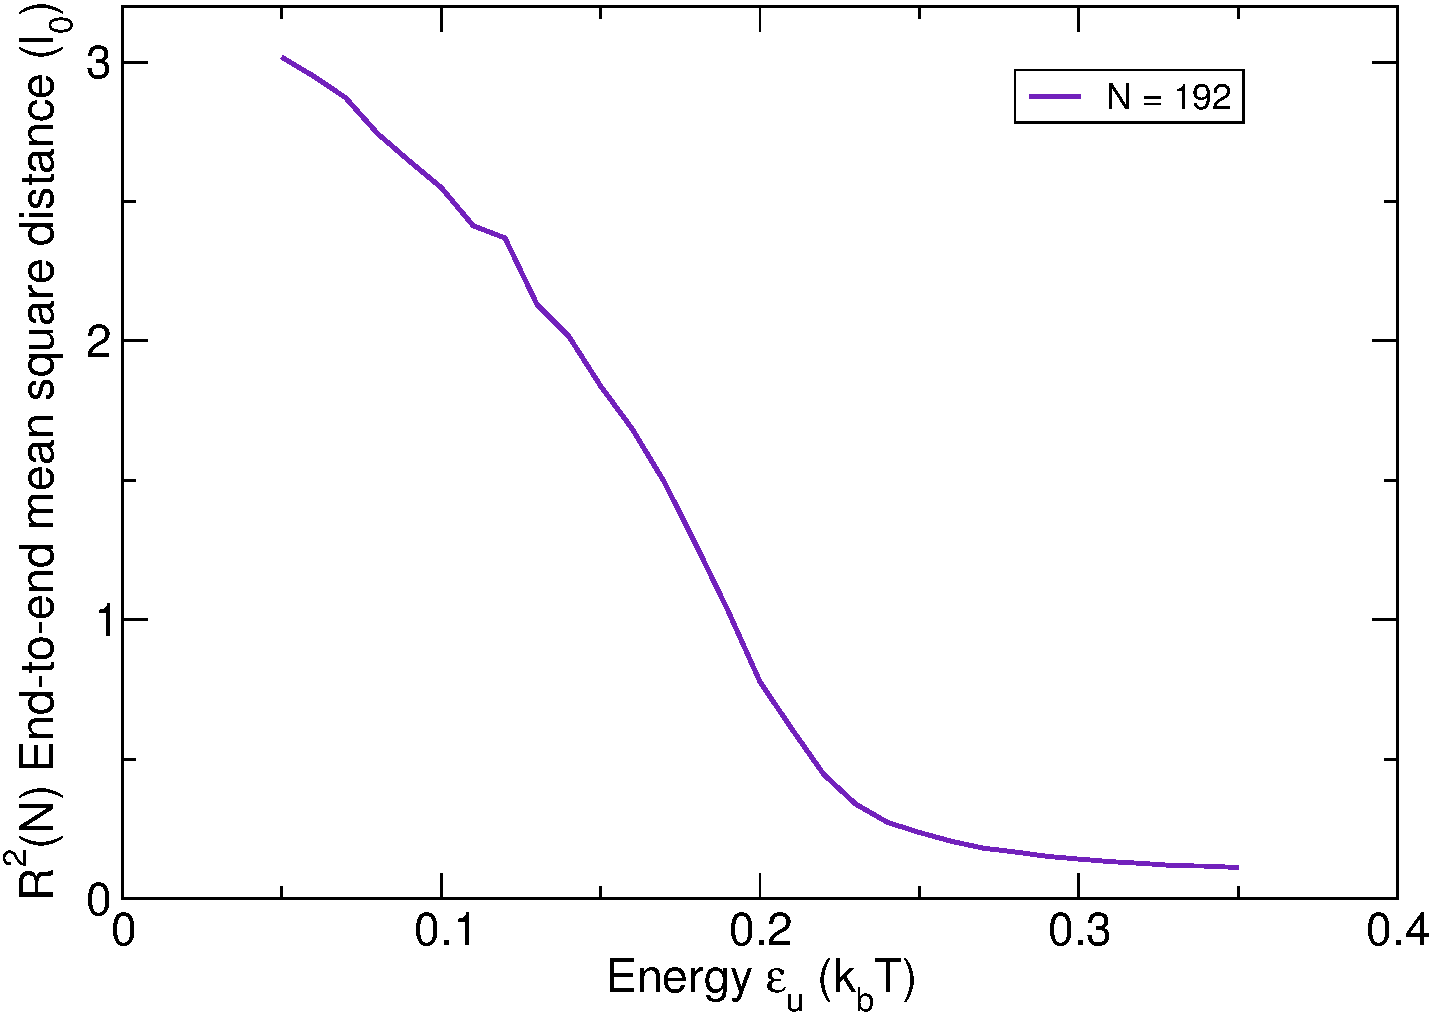
\includegraphics[width=9cm]{collapse}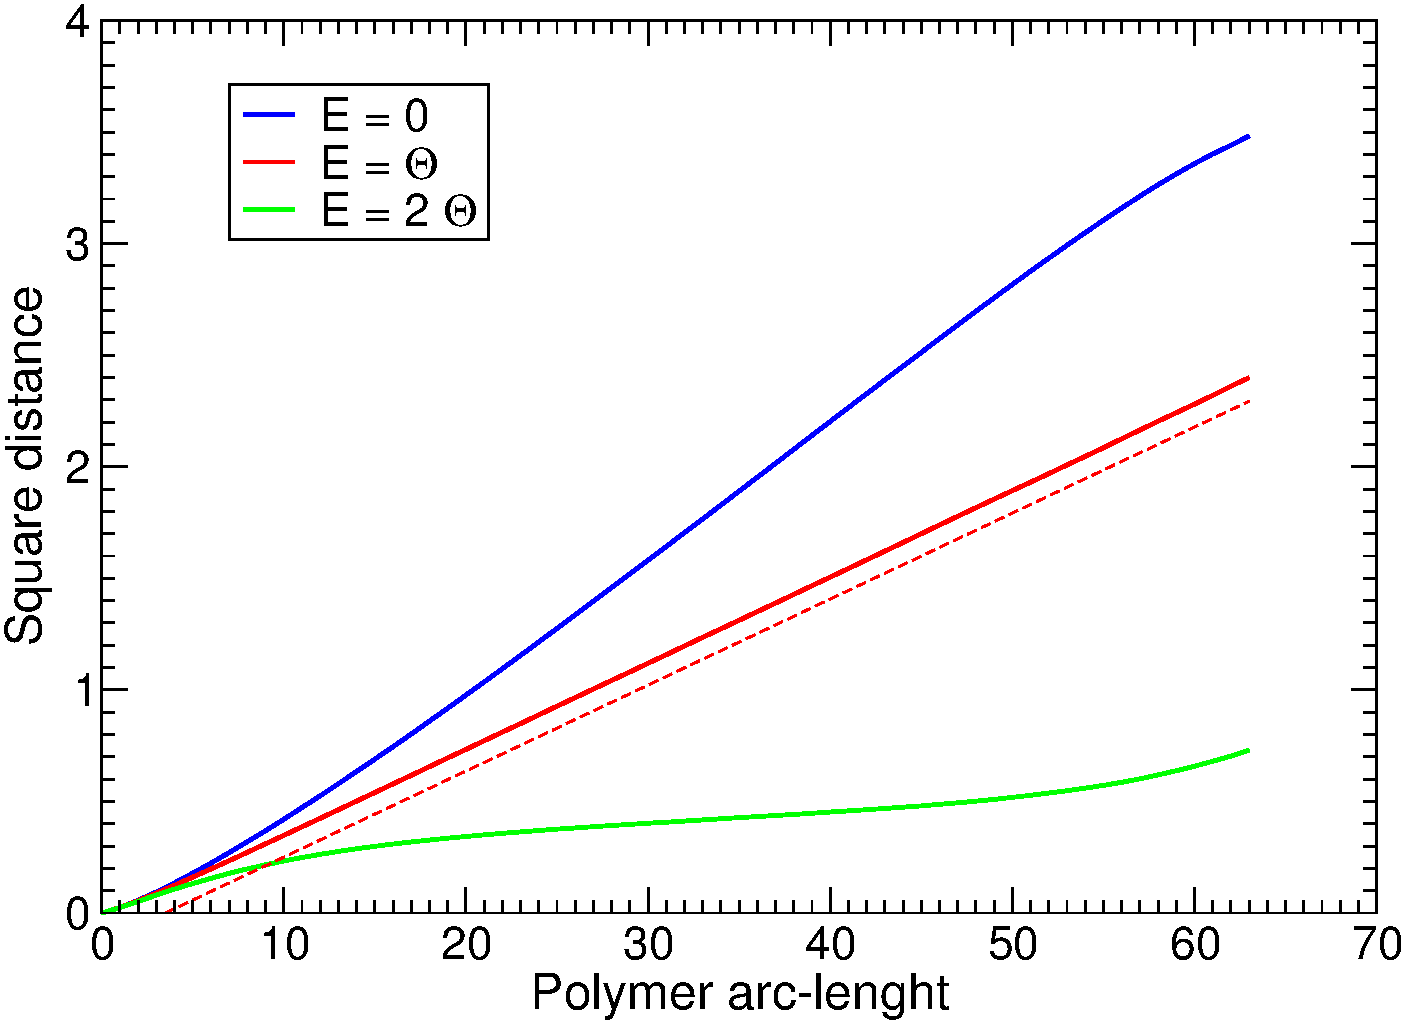
\includegraphics[width=9cm]{merrUno}\\
\caption{Coil-globule transition: The left graph shows that the size of the
  polymer which is in  function of the fluctuations of the end-to-end
  distance $\langle \vec r^2 \rangle$ undergoes a transition from a coiled
  state to a globular state as a function of the interaction energy
  $\epsilon_u$. The right picture shows the behaviour of the mean
  square distance as a function of arc-length distance at different
  values of interaction energy $E$, for chain length
  ($N = 64$). The relation is linear at the $\Theta$ energy in evident
  agreement with the mean field implication that $F_{flory} =
  F_{ideal}$ at $\epsilon_u = \Theta$. Coil and globular behaviours
  are found for respectively lower and  higher interaction
  energies. In the limit-case of $E = 0$ the polymer is a coil fractal
  with measured exponent of $R \propto N^{0.598}$ in remarcable
  agreement with Flory-Huggins theory predictions
  (Eq. \ref{eq:volcoil}). The two plots have been obtained using as
  parameters $\hat \lambda = 0.19$, $\hat \sigma = 0.1$, $\hat \alpha
  =0.3$, parameters with hat are in units of $l_0$.}
\label{fig:collapse}
\end{figure}

In order to understand the coiled state we can calculate the equation
of state of the interacting polymer:
\begin{equation}
  P = - \frac{\partial F}{\partial V} = \left( - \frac{5}
      {3 \lambda^2 N} V^{2/3} + \frac{N(N-1)}{2} 
      \frac{v}{V} \right) \cdot \frac{k_b T}{V}.
\end{equation}

Under those conditions, this equation sets the mean size of the coiled
polymer, assuming $v$ positive, $P = 0$ and taking the leading term in
$N$ we obtain:
\begin{equation}
  V = \left( \frac{3}{10} v \lambda^2 \right) ^{3/5} N^{9/5} \qquad 
  \mathrm{or} \qquad R \propto N^{3/5}
\label{eq:volcoil}
\end{equation}
which sets the scaling of the size of the coiled polymer as a function
of the polymer length in remarcable agreement with simulation
results (see Fig. \ref{fig:collapse}).

In our model the length of the Nucleoid is a fixed parameter, so we
are not interested in the scaling of the size with length but instead
in renormalizing the paramiters so that the size remain fixed despite
of the number of beads $N$ we use to represent the the polymer. The
physical size $V$ in units of ${l_0}^3$ can be rewritten as:
\begin{equation}
  \frac{V}{{l_0}^3} = \left( \frac{1}{2{l_0}^3} v N^2 \right)^{3/5}.
\end{equation}
We impose this value to be constant for different $N$, this sets the
scaling of $v$ as a proportional to a effective volume parameter
$\nu \equiv v N(N-1) \approx v N^2$ which is carachteristic of the
physical system of polymer and solvent and not of the details of the
simulation. Since this physical parameters can be written by the
following formula:
\begin{equation}
  \nu = \frac{4}{3} \pi N(N-1) (\Theta - \epsilon_u)
  (\alpha - \sigma).
\label{eq:nuvolume}
\end{equation}
the scaling of the simulation parameters $\sigma$, $\alpha$
and $\epsilon_u$ are still not univocally determinated.

A definitive explanation of the scaling behaviour can be given only by
making an argument about the size of the polymer in the globular
phase: for very large attractive energies or for large pressures the
polymer will collapse on his excluded volume, and become
incompressible. Since the total excluded volume in the simulations is
proportional to the number and the size of the beads
$N \sigma^3$ the excluded volume parameter $\sigma^3$ should scale as
the inverse of $N$ in order to keep the size of the globule constant
and indipendent on the number of beads. The attraction volume
parameter $\alpha^3$ should behave the same in order to keep $\Theta$
constant. From equation \ref{eq:nuvolume} then we can interpret the
scaling of the interaction energy $\epsilon_u$.
This argument lead to the {\it second, third and fourth rule of
  parameter normalization}:
\begin{equation}
   \frac{4}{3} \pi \sigma^3 =  \Sigma / N \qquad \mathrm{and} \qquad 
   \frac{4}{3} \pi \alpha^3 =  A / N \qquad \mathrm{and} \qquad 
   \epsilon_u - \Theta \equiv \Delta  \epsilon_u = 
  \Delta E_u / (N - 1).
\label{eq:sigmarin}
\end{equation}

The rules of parameter normalization set the hard core repulsion
volume $\sigma^3$ and the volume of interaction $\alpha^3$
proportional to physical volumes which can be considered global
observable characteristic of the specific polymer being simulated
($\Sigma$ and $A$). In the same way the difference between attraction
energy per beads and the theta energy $\epsilon_u - \Theta$ is
proportional to a physical internal energy $\Delta E_u$ which is
positive for collapsed polimers and negative for coiled ones. Using
this notation, the effective volume parameter can be written as
$\nu = - \Delta E \left( \Sigma - A \right)$.

The simulation parameters $\sigma^3$, $\alpha^3$ and $\Delta
\epsilon_u$ are inverse proportinal on the number of beads
$N$; those parameters can thus be respectively interpreted in the most
intuitive way as excluded volume, interaction volume and internal
energy per unit bead (or link). The total excluded volume $\Sigma$,
the total interaction volume $A$ and the total internal energy $\Delta
E_u$ are thus by definition extensive variables of the system.

Also, those rules of parameter normalization show also a
limitation in our simulations: the shape of our interaction potential
fixes $\epsilon_u$ to be defined positive, the scaling law for
the difference between this parameter and the critical energy $\Theta$
thus fixes a lower limit to the simulable internal energy which
depends on the resolution $N$ fixed by the following indetermination
relation:
\begin{equation}
\Delta E_u \cdot \Delta s > - \Theta L,
\label{eq:indetermination}
\end{equation}
where $\Delta s \equiv L (N-1)^{-1}$ is the link arc-length and
is inverse proportional to the degree of discretization, $L$ is the
polymer length.
%A part the obvious parallel with the discretization
%of the action of trajectories in quantum mechanics
The practical
meaning of this realation is that in order to simulate configurations
of coiled polymers with large negative internal (repulsive) interaction
$-\Delta E_u$, we will be forced to increase the number of beads $N$ 
(details) accordingly.

The implementation of the fourth rules of parameter
normalization (summarized in table \ref{tab:renor}) is an instrument
which let us to remove the dependence of the free energy from the
number of beads $N$. As a result we have a theory which gives us
consistent results for simulations runned at different $N$.

\begin{table}[h]
\centering
  \begin{tabular}{c|c|c|c|l}
    {\bf \# } & {\bf (1) } & {\bf (2) } & {\bf (3)} & {\bf (4)}\\
\hline
$1^{st}$ & $\lambda$ & $l_0$ & 
  $\lambda = l_0 \sqrt{\frac{5}{3} \frac{1}{N}}$ &
  Mean end-to-end distance at $\Theta$ transition \\
$2^{nd}$ & $\sigma$ & $\Sigma$ &  $\sigma^3 = \frac{3}{4\pi} \Sigma / N$ &
  Hard core repulsion volume \\
$3^{rd}$ & $\alpha$ & $A$ & $\alpha^3 = \frac{3}{4\pi} A / N$ &
   Interaction volume\\
$4^{th}$ & $\Delta \epsilon_u$ & $\Delta E_u$ & $\Delta  \epsilon_u = \Delta
E_u / (N - 1)$ &
   Total internal energy\\
  \end{tabular}
  \caption{Rules of parameter normalization: (1) Simulation parameter,
  (2) Physical observable, (3) Scaling, (4) Interpretation}
  \label{tab:renor}
\end{table}

\begin{figure}[h!]
\centering
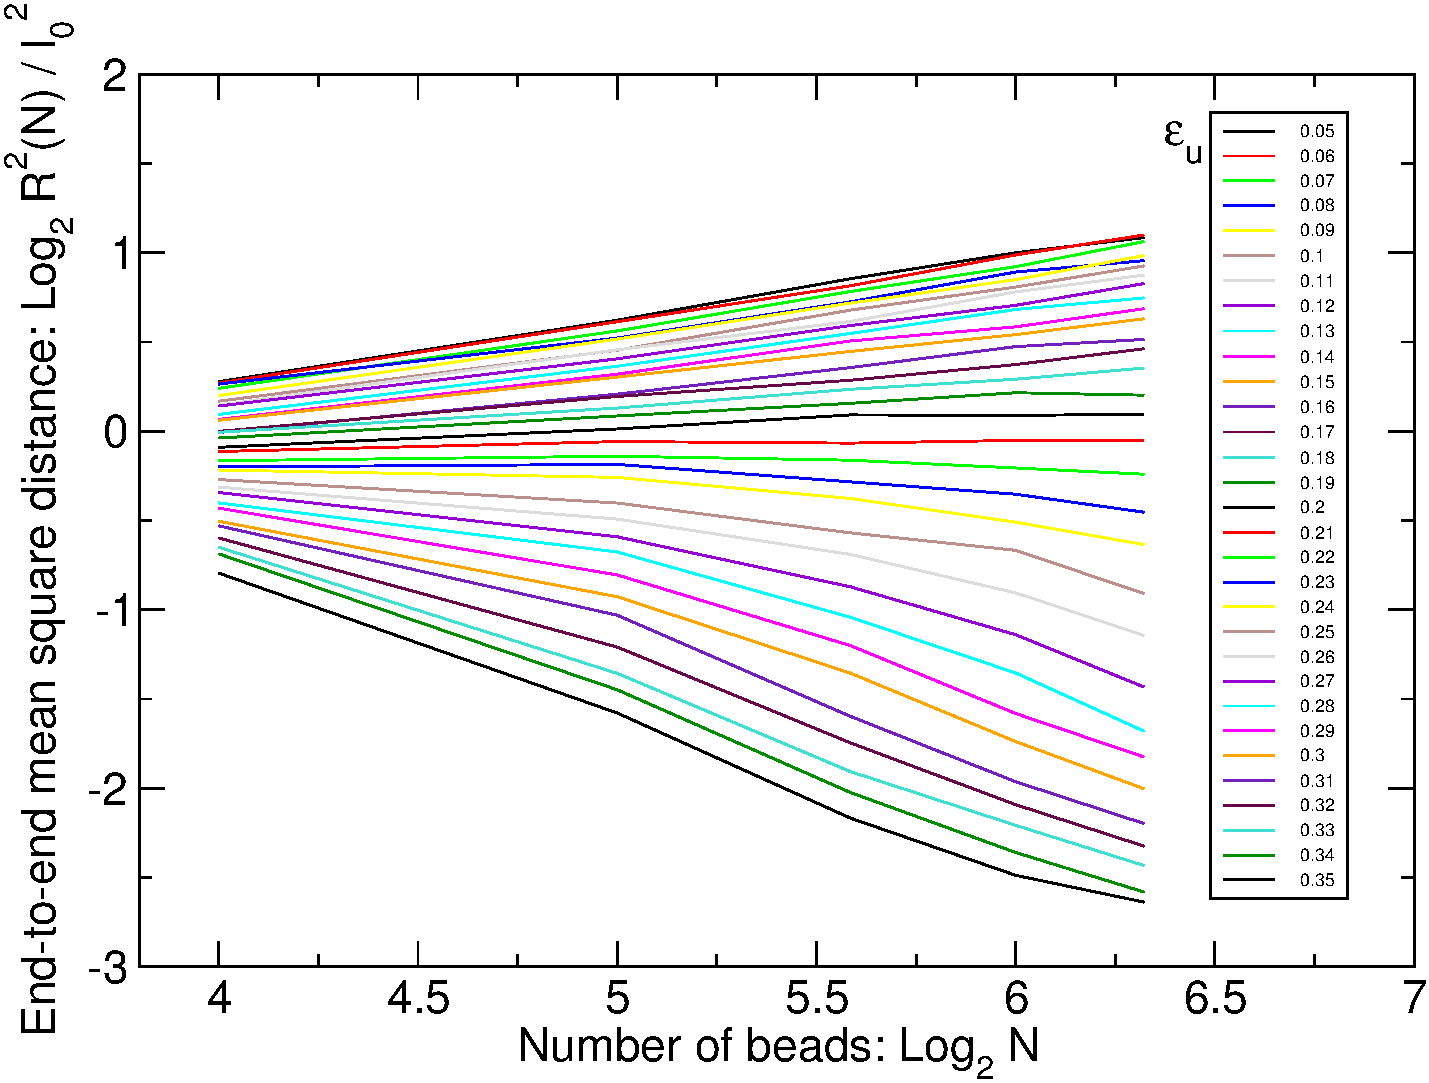
\includegraphics[width=9cm]{ssK}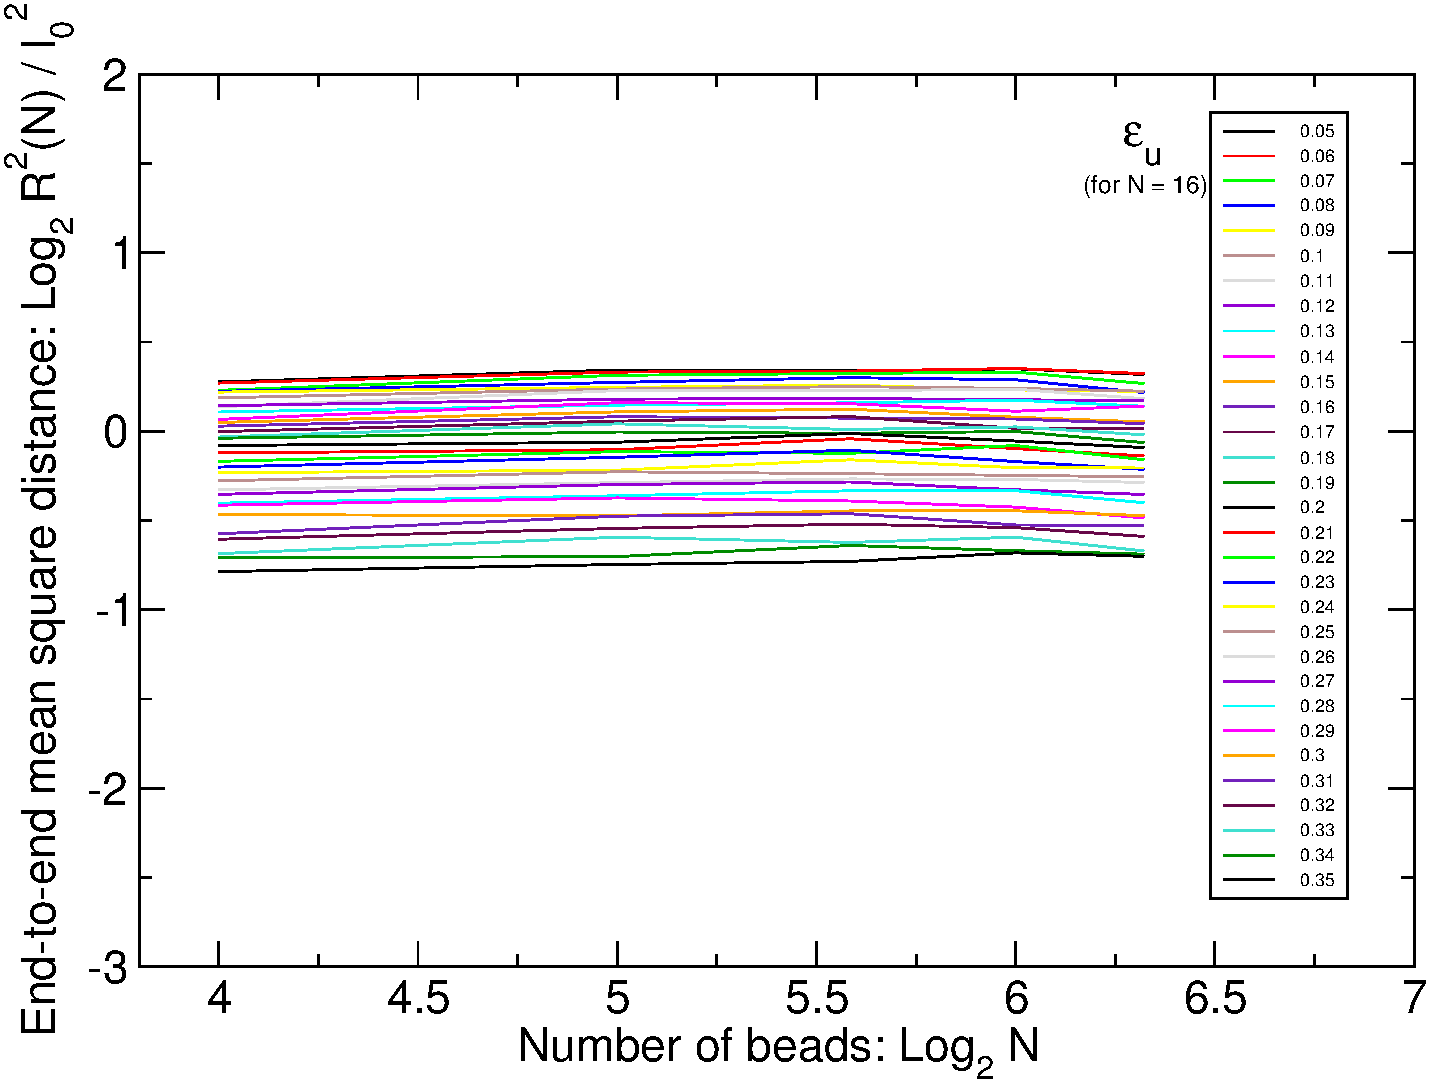
\includegraphics[width=9cm]{ssL}\\
\caption{Parameter normalization:
  end-to-end mean square distance as a function of the number of beads
  after application of the first three rules of parameter
  normalization (left graph) and after application of all four rules
  of parameter normalization (right graph). The graphs are the result
  of simulations using our algorithm and are made for
  different interaction energy parameter $\epsilon_u$ for a range
  which span the coil-globule transition. For a summary of the rules
  see table \ref{tab:renor}. The left graph is necessary in order to
  find the critical energy (straight line for $\epsilon_u = 0.21$)
  while the right graph shows that after proper normalization of the
  parameters the number of beads is a free parameter $N$ of the
  simulation which doesn't influence in a significant way the physical
  observable of the end-to-end square distance as a function of
  $\epsilon_u$.}
\label{fig:renor}
\end{figure}

\begin{figure}[h!]
\centering
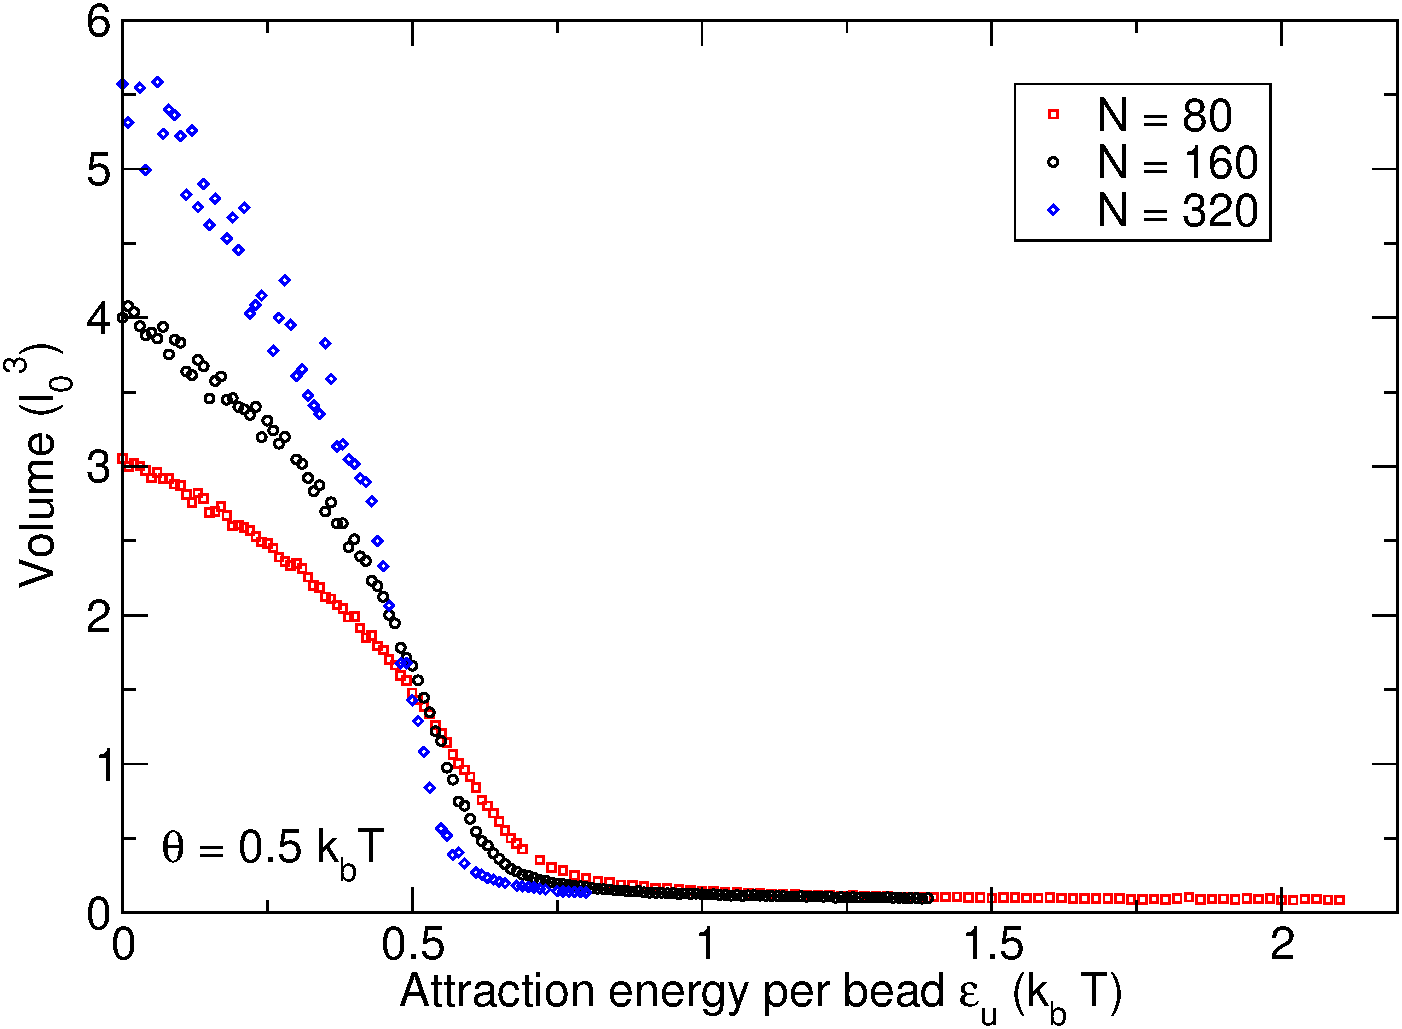
\includegraphics[width=9cm]{reno_before}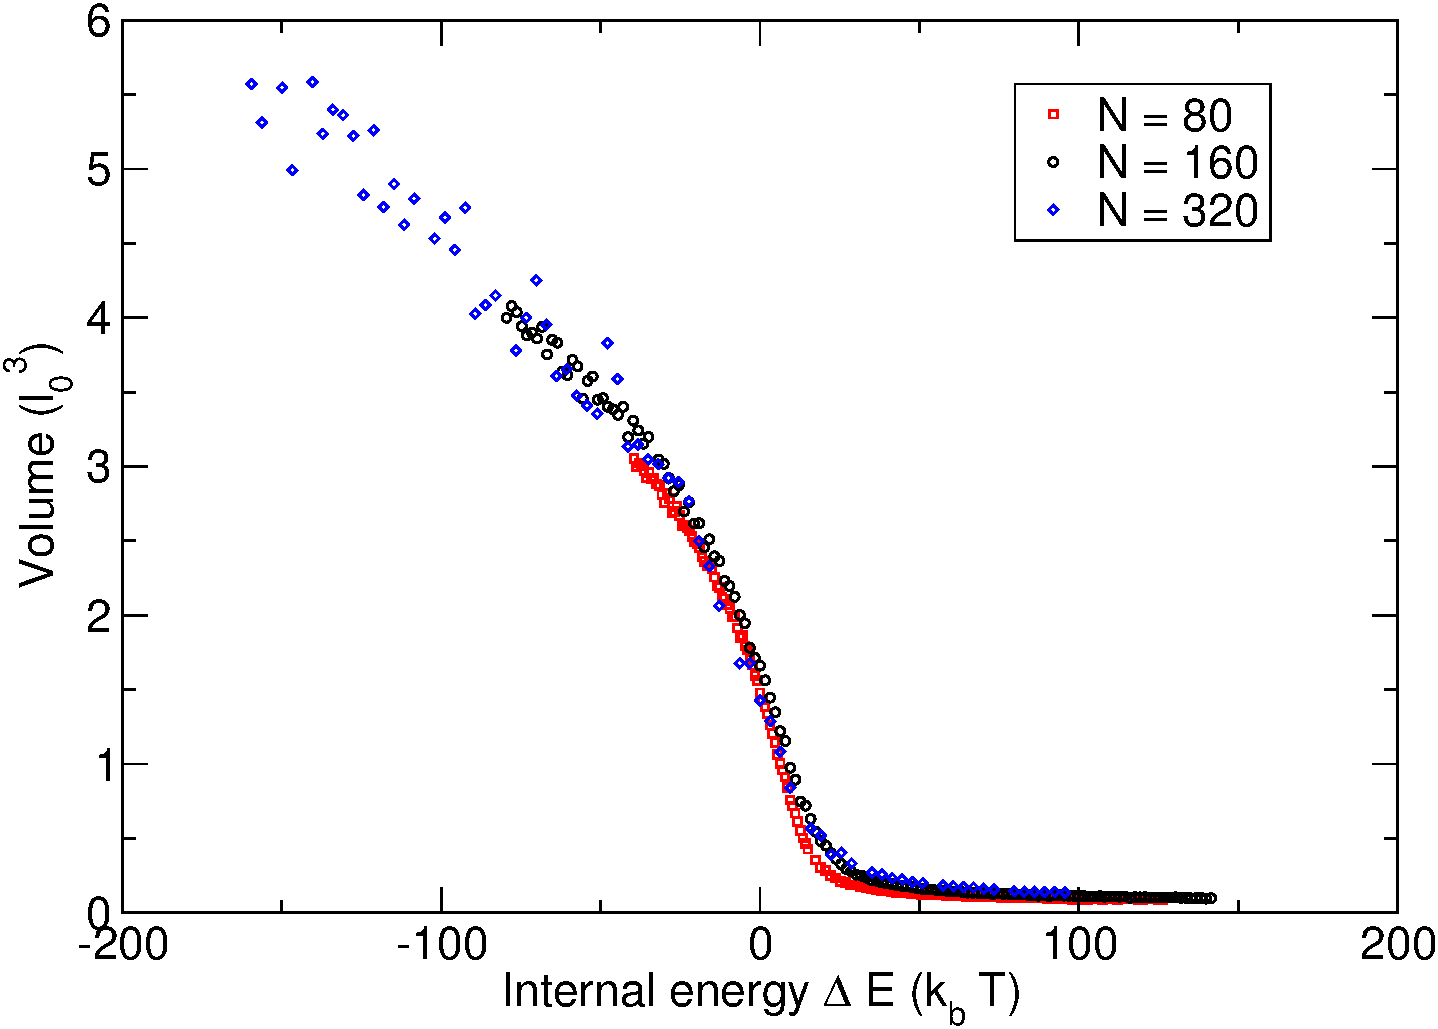
\includegraphics[width=9cm]{reno_after}\\
\caption{Parameter normalization:
  collapse diagram (Volume as a function of interaction energy) for the
  same polymer ($\Sigma = 0.1 {\l_0}^3$ and $A = 6 \Sigma$) with
  different discretization parameter $N$. The left graph is
  after application of the first three rules of parameter
  normalization. The right graph is after application of the fourth
  rule. From the left to the right graph the following two operations
  have been applied: $x \to x - 0.5$, $x \to (N - 1)x$.}
\label{fig:renor}
\end{figure}

Using only the global observables $(V, A, \Sigma, \Delta E_u, T)$ we can
obtain the renormalized Flory free energy for the coiled state:
\begin{equation}
  F_{coil} =   F(0) + \frac{3}{2 {l_0}^2} k_bT V^{2/3}
  - k_b T \frac{\Delta E_u}{k_b T} \frac{A - \Sigma}{V},
\label{eq:coilen}
\end{equation}
with equation of state:
\begin{equation}
  P = \left( \frac{V^{2/3}}{{l_0}^2} + \frac{\Delta
      E_u}{k_b T} \frac{A - \Sigma}{V}
      \right) \cdot \frac{k_b T}{V}, \quad
    \mathrm{and} \quad
  V_{coil} = \left( {l_0}^2 
    \frac{- \Delta E_u}{k_b T} \right)^{3/5}
  \left( A - \Sigma  \right) ^{3/5} \quad \mathrm{unconfined.}
\end{equation}

A peculiar property of this last relation is the monotonical growth of
the volume as a function of the effective renormalized interaction
energy $-\Delta E$. One could think from this relation that the
fluctuation of the coil end-to-end distance can grows indefinely in
function of this parameter, this is not true since relation
(\ref{eq:indetermination}) fixes an upper bound for this parameter for
any finite number of statistical elements $N$ and in turn for any
finite $N$ the polymer is confined in a finite volume $V$ of the
space. In turn this is a realistic description of a
self-interacting {\it single} polymer, since the swelling is limited
not only by the ultraviolet natural cutoff given by the Kuhn length
but also by the length of the polymer. In comparison to previous
works\cite{}, the model doesn't aim at a description of the
``thermodynamic limit'' $N \to \infty$, in which the polymer can be
described by the self avoiding walk model \cite{Degennes1979}.

The free energy in the virial expansion elaborated by Flory lets us
predict the size of the coiled phase, the existence of a critical
energy of transition and the formula of the order parameter. Thus it
helped us to write rules of parameter normalization which let use
keep the discretization of the problem $N$ as a free parameter. On the
other end this approach alone fails to describe the globular phase and
the transition from ideal to globular state.

% \subsection{Fractal structure of the coiled polymer}

% The coiled state of the polymer is considered a fractal state since it
% fills the space in the same way over a large range of length
% scales. As depicted in Fig. \ref{fig:collapse} and predicted by Flory
% theory the relation between the end-to-end radius and the arc-length
% distance between two beads scales as $R \propto N^{3/5}$. While this
% is true for large arc-length distance, a detailed analysis of
% Fig. \label{fig:collapse} for the coiled state shows in fact a
% crossover between a region $s < \xi_T$ where the polymer behaves as a
% random coil and a region $s > \xi_T$ where it behaves as a coiled
% fractal.

% The theory for explaining this crossover have been studies in the '70s
% by DeGennes. He identified the size of the thermal blob at which the
% crossover happen as the length scale at which excluded volume
% interactions are of the order of $k_b T$. The relation can be written
% as:
% \begin{equation}
% k_b T \left| \nu \right| \frac{{g_T}^2}{{\xi_T}^2} \approx k_b T
% \end{equation}
% where $g_T$ is the number of beads in a thermal blob and $\nu$ is the
% effective excluded volume defined by eq. \ref{eq:nuvolume} in our
% model.

\subsection{The globular phase}

In the globular phase ($\epsilon_u > \Theta$, $\Delta E_u > 0$, see
equation \ref{eq:theta}) the effective volume
becomes negative. In this conditions the polymer start to collapse and
the second order virial expansion is not enough to find the
equilibrium mean size. An approximate model for the size of the
globule can be obtained by using a third order expansion for the free
energy although this approach seems an ad hoc hypotesis and in fact it
fails to catch important properties of the globular state.

In order to derive a good formula for the free energy in the globular
phase, we can study the plots of the square distance of beads in
function of the arc-length in the globular phase using our
simulations. The typical results for such a plot follow the shape of
the green line in the right graph of Fig. \ref{fig:collapse}: the
square distance grows linearly for very short arc-lenghts, then, at
arc-lenght bigger than a characteristic length which depends on
the interaction energy, the distance plateau.

An explanation of the linear growth for short arc-length distance is that
the polymer behaves as a random walk trying to find his way out of the
crowded environment made by himself, the interactions are thus
screened for small distances. For larger arc-length distances
the polymer reaches the globule surface and thus return in
the inside of the globule, it is at this point that the distance in
function of the arc-length plateaus.
%% Give a formula for the size of the globular blob ?

At arc-length distances greater than the interaction screening length,
the correlations between the positions of the beads are
null which means that the information about the existence of a link
network is totally lost. This suggest the form of the free energy of
the globule:
\begin{equation}
F_{globule} = F(0) - k_b T C \log \left( \frac{V - \Sigma}{{l_0}^3} \right).
\end{equation}
where the volume $V$ depends on the pressure, energy of interaction
and temperature $V = V(P, E_u, T)$ and $C$ is a numerical
parameter which should contain the number of degree of freedom of the
system and hypotetically can depend on other variables. This is the
formula for the free energy of a confined gas: we choose this formula
because the polymer behave as a gas if the information of the link
network is lost for big enough arc-length distances.

The free energy of the globule have some important features. For
volumes which are smaller than the hard core repulsion volume $\Sigma$
the argument of the logarithm becomes negative, also the free energy
diverges for $V \to \Sigma$ which means that for big enough attractive
energies $E_u$ the polymer becomes incompressible like a liquid.

\subsection{Free energy of the real polymer}

Now that we know how the free energy can behave in the two limiting
cases of coil and globular phase, we can write down the free energy
for the real polymer which catch the incompressible globular state and
describe the transition from coil to globule as the most simple
interpolation formula between the two. We do this by arbitrarily
choosing:
\begin{equation}
  F_{real} = F_{coil} + F_{globule},
\end{equation}
and setting the following constraints:
\begin{equation}
  F_{real} \to F_{coil} \ \ \mathrm{for}\ \ V \to \infty
  \qquad \mathrm{and} \qquad
  F_{real} \to F_{globule} \ \ \mathrm{for}\ \ V \to \Sigma;
\end{equation}
which set the value of the $C$ parameter. Finally we obtain:
\begin{equation}
  F_{real} = F(0) + \frac{3}{2 {l_0}^2} k_bT V^{2/3}
  - k_b T \left[ \frac{\Delta E_u}{k_b T} \frac{A - \Sigma}{V}
  + \frac{\Sigma}{V} \right]
  - k_b T \log \left(\frac{V - \Sigma}{{l_0}^3} \right).
\label{eq:enreal}
\end{equation}

This formula can be regarded as a mean field argument for the polymer
free energy where the parameter of our simulation appear
explicitly. This formula converges to the one proposed by Flory for
the coiled state and is also able to describe the collapse to the
globular state. This also let us calculate an equation of state for
single polymer which can eventually be used in microfluidic experiments:
\begin{equation}
  P = \left[ \frac{V^{2/3}}{{l_0}^2} +
    \frac{\Delta E_u}{k_bT} \frac{A - \Sigma}{V} + 
    \frac{\Sigma}{V} - \frac{V {l_0}^3}{V - \Sigma}
  \right] \cdot \frac{k_b T}{V},
\label{eq:realestate}
\end{equation}
our simulations run without confinement, we can thus solve implicitly
for the size of the polymer $V(P,\Delta E_u,T)$ as a function of the
interaction energy $E_u$ by setting the pressure to zero
$P(V, \Delta E_u, T) = 0$, obtaining the plot in figure
\ref{fig:colreal}. This prediction show remarcable agreement with the 
the results of the simulations (Fig. \ref{fig:colrealsim}).

\begin{figure}[h!]
\centering
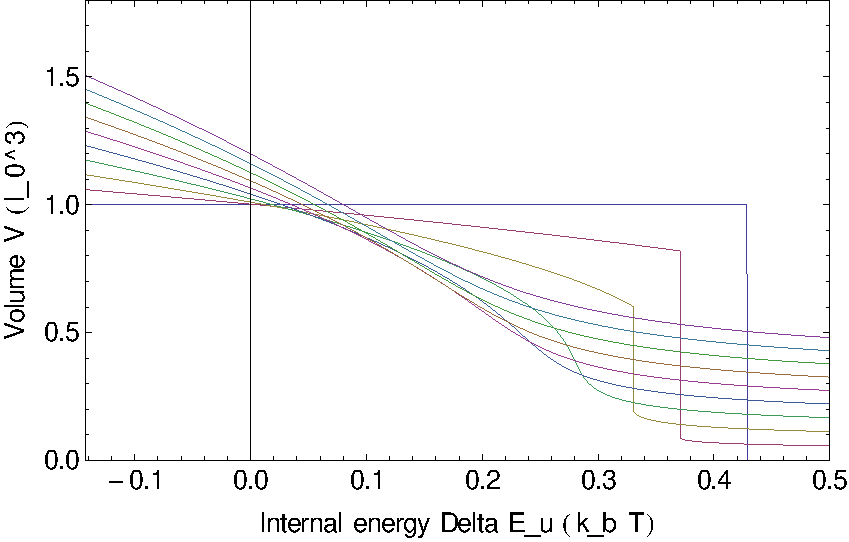
\includegraphics[width=9cm]{colrealAS}
\caption{Phase diagram of the size of the polymer $V(P,\Delta E_u,T)$ in
  function of the interaction energy $\Delta E_u$ at $P = 0$ and $T = 
  \mathrm{const}$. The lines are obtained solving Eq.
  \ref{eq:realestate} using numerical methods at different value of
  hard core repulsion parameter $\Sigma$ and $A = 8 \Sigma$.}
\label{fig:colreal}
\vspace{5mm}
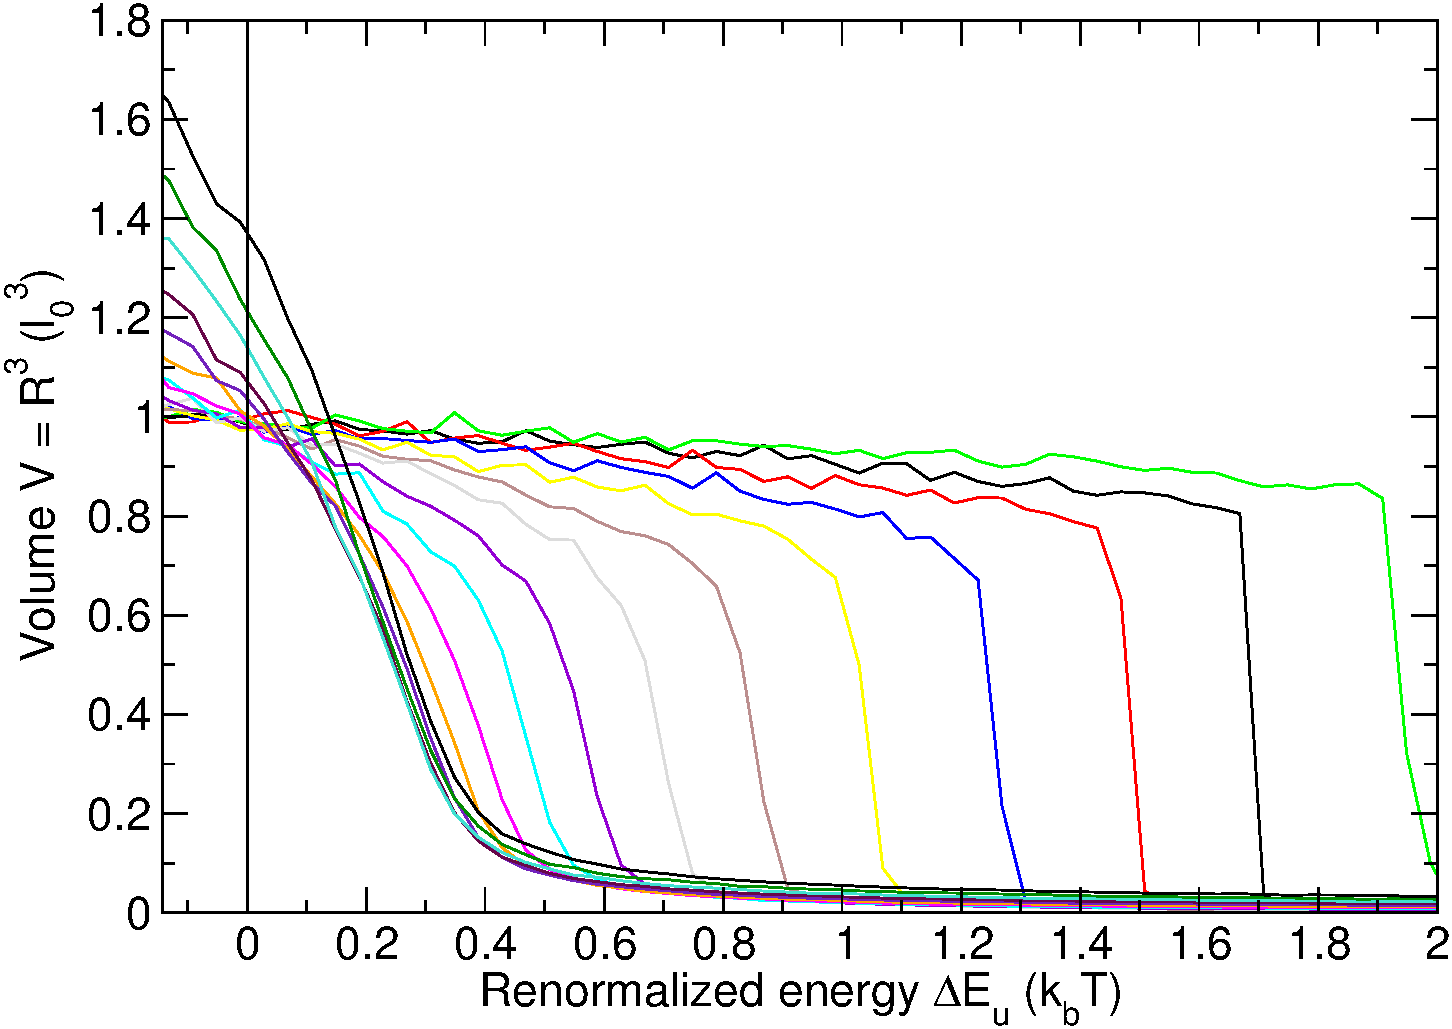
\includegraphics[width=9cm]{colrealSIM}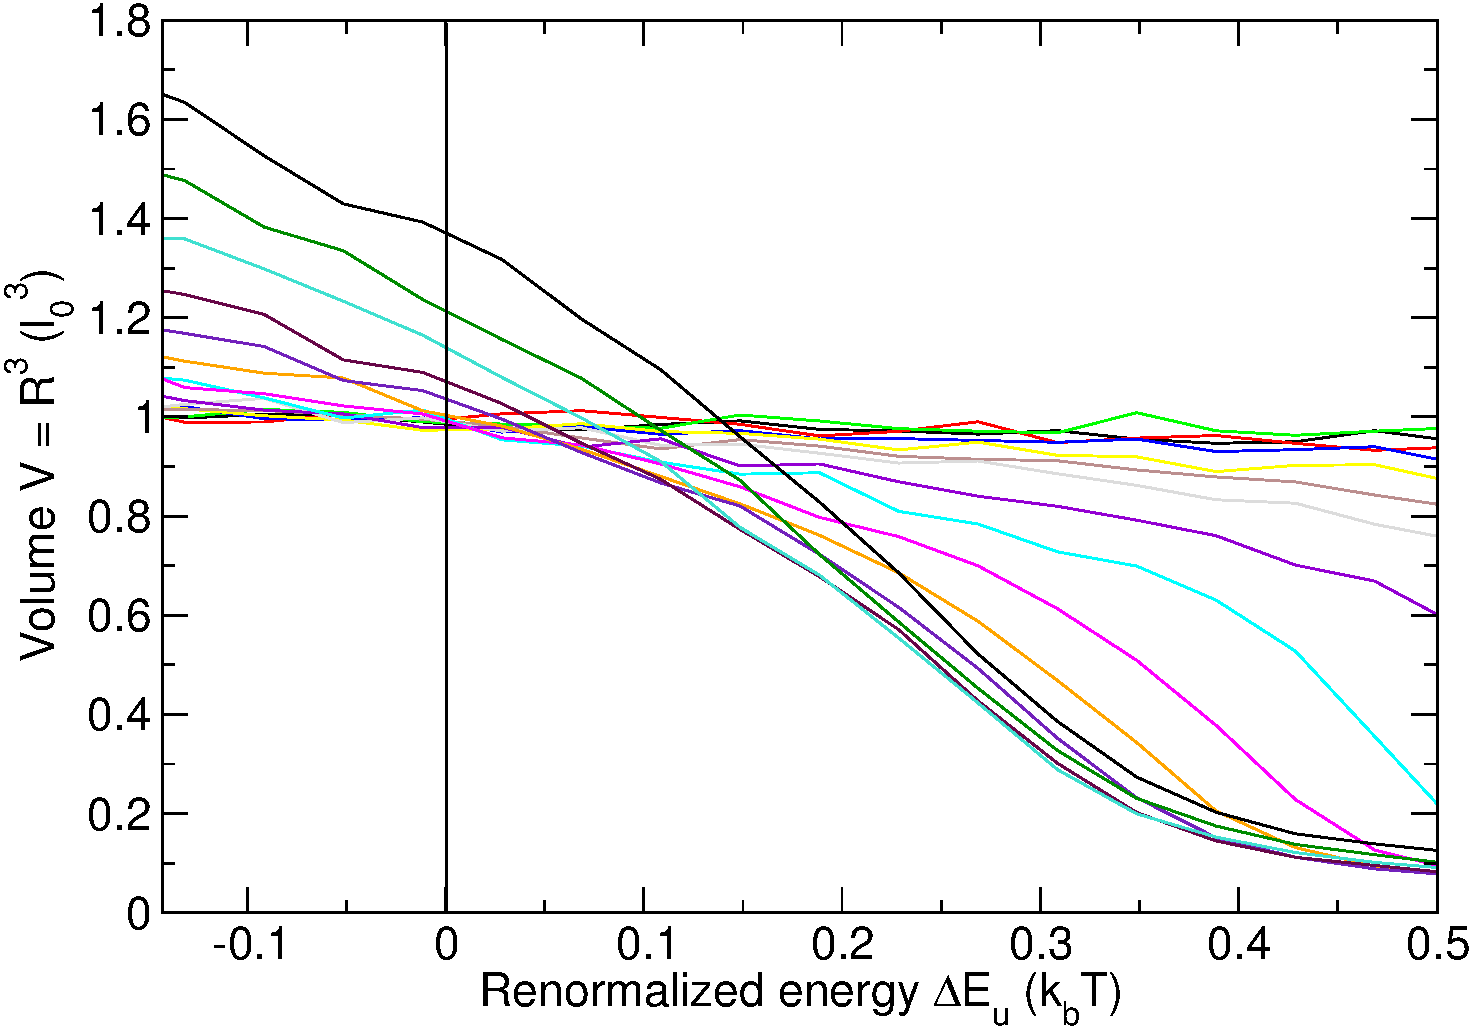
\includegraphics[width=9cm]{colrealSIMsmall}\\
\caption{Phase diagram of the size of the polymer $V(P,\Delta E_u,T)$ in
  function of the interaction energy $\Delta E_u$. The lines are
  obtained by simulating the polymer at different value of hard core
  repulsion parameter $\Sigma$ and $A = 3 \Sigma$, the abscissa is
  rescaled. The graph on the rigth is a zoom of the graph on the left
  for comparison with the theoretical predictions.}
\label{fig:colrealsim}
\end{figure}

It is evident that this results defines a critical globular volume
$\Sigma_c$. For $\Sigma > \Sigma_c$ (Big globule) the transition is
the well studied second order $\Theta$ transition while for $\Sigma <
\Sigma_c$ (Small globule) the coil-globule transition is sharp
(first-order type) and the energy moves at greater values then
$\Theta$. This phenomenology is in agreement with the description of
the $\Theta$ transition given by Lifshitz in 1978 though obtained with
different methods\cite{Lifshitz1978}. We show a schematical phase
diagram as a function of the parameters in figure \ref{fig:unifphas} in
order to explain the phenomenology.

\begin{figure}[h!]
\centering
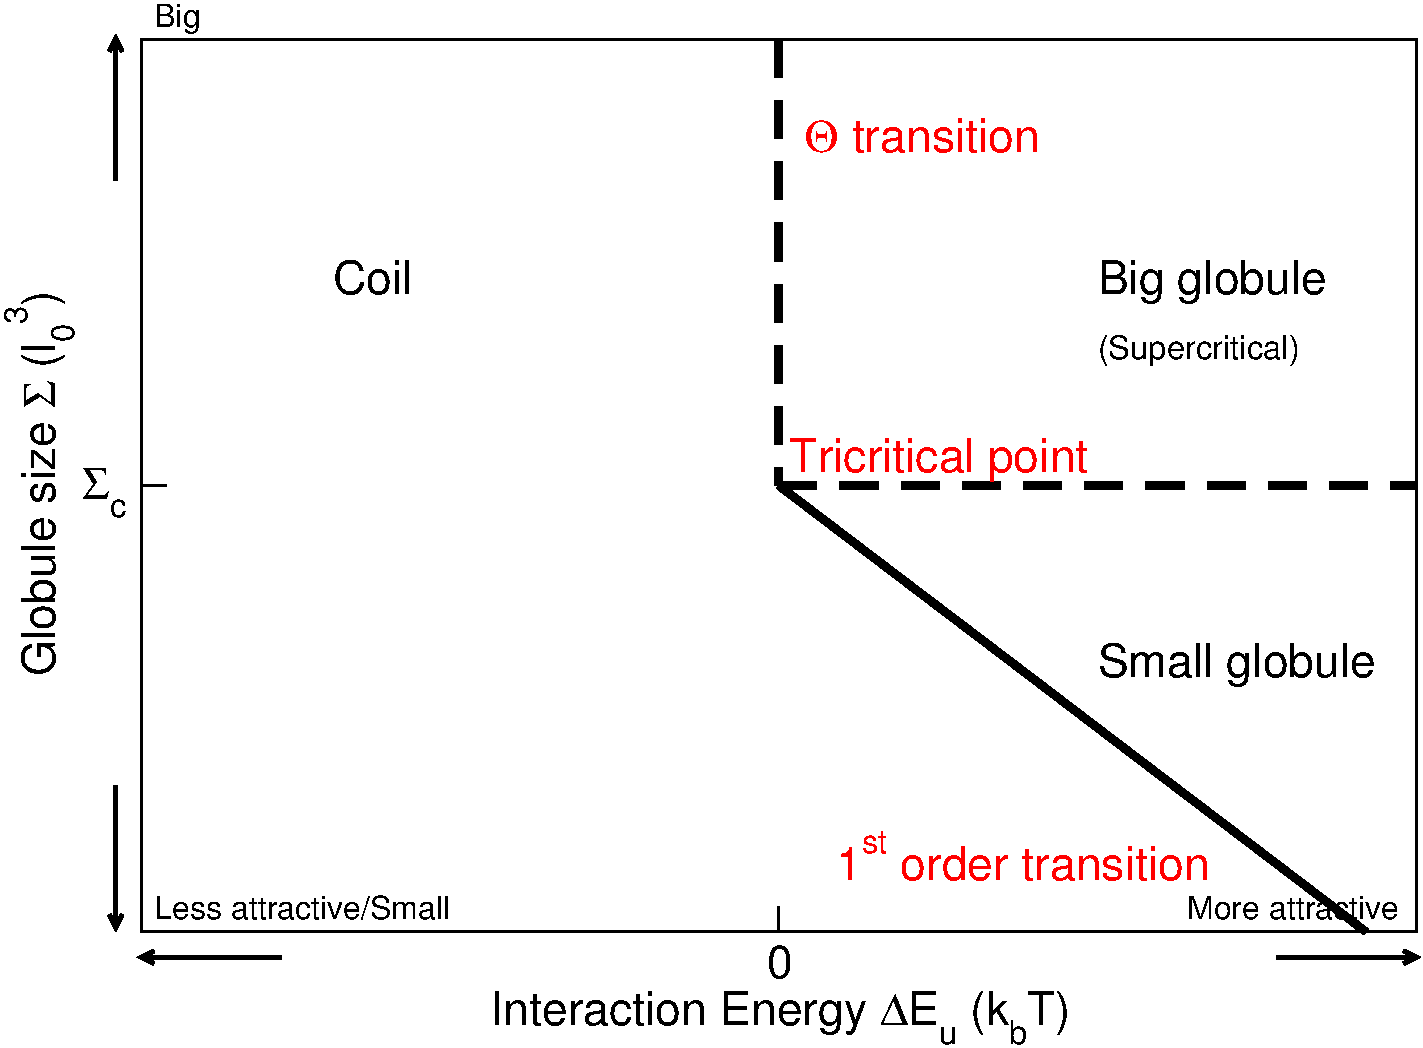
\includegraphics[width=9cm]{uniform_phases}\\
\caption{Parameters phase space as a function of uniform interaction
  energy $\Delta E_u$ and volume of globular phase $\Sigma$.}
\label{fig:unifphas}
\end{figure}

\section{Extimation of the parameters for \ecoli nucleoid}

In this paper we are interested in modeling the behaviour of the
\ecoli nucleoid in different enviromental conditions. We will thus
keep the interaction energies $\Delta E_u$ and $\Delta E_l$ and the
configuration of the localized interactions free and instead extimate
and fix the volume parameters $(l_0, \Sigma, A)$.

A rough extimate those parameters can be done with different
approaches:
\begin{itemize}
\item
The first approach would be to take as a comparison a Worm-Like-Chain
with the length, the persistence length and the volume radious of the
DNA molecule of the \ecoli chromosome, and from this simplified model
extract an extimate of the parameters for the nucloid; this would give
us a very inaccurate extimation because we would neglect the RNA and
proteins bounded to DNA as well as the global effect of the molecule
supercoiling and topology which are currently not extimable.
\item
The second approach would be to extract the observed global parameters
from recent experiments performed on purified nucleoids under optical
microscopy, in this case we would introduce an experimental
due to the difficulty of identifying the theta transition.
\end{itemize}

\subsection{Comparison to a Worm-like-chain}
An extimate of the end-to-end distance of the nucleoid at $\Theta$
transition $l_0$ in nanometer can be given by taking as a comparison
the the end to end distance for a Worm-Like-Chain which can be
approximated for long chains by the formula:
\begin{equation}
{l_0}^2 = 2 l_p L
\end{equation}
where $L$ is chain contour length and $l_p$ is the persistence
length in nanometers. Substituting the contor length of \dna in \ecoli
nucleoid  ($\sim 1.577 mm$) and the persistence length of naked \dna
in physiological conditions ($\sim 50 nm$) we obtain
\begin{equation}
  l_0 = 12.85 \mu m.
\end{equation}

The excluded volume $\Sigma$ can be rougly eximating by calculating
the volume of the cylinder containing the \dna molecule as if it was
straight using the formula:
\begin{equation}
\Sigma = (\pi / 2) d^2 L
\label{eq:sigmaS}
\end{equation}
where $d$ is the \dna diameter taken by the sum of the \dna Helix
Diameter $(23.7 \mathrm{\AA})$ and two times the \dna screening length
in physiological condition $(\sim 4\nm)$. We obtain for the excluded
volume:
\begin{equation}
  \Sigma \sim 0.1 \mu m^3 \sim 5 \cdot 10^{-5} {l_0}^3
\end{equation}

This number is calculated by considering the
volume of a {\it naked} B-\dna double helix, which mean without any
{\it protein} attached and no plectonemic or secondary
structures. Those effect could increase the excluded volume of the
\dna in-vivo conditions.

\subsubsection{Attraction box}
% add references from shacknovich psi transition
In our model beads interact with each other by their repulsive
excluded volume force and by an attractive uniform force which we
assume is due to the molecular crowding of the cytoplasm. The
depletion of the molecules in the cytoplasm due to the presence of the
long \dna macromolecule results in an effective attraction between
couples of \dna double Helix segments. This effect
have been recently shown in \dna and PET solutions
\cite{Kojima2006} and has been advanced as a possible
driving force of chromosomal organization\footnote{
  In their work, the Cook group doesn't investigate the coil
  globule transition but they focus on \dna looping instead, in the
  cited paper Marenduzzo states ``There are entropic costs associated
  with forming \dna or chromatin into a loop, but these can be overcome
  if large enough complexes are bound to the template'' which assumes
  that depletion forces are excerted on the \dna through large enough
  complexes.}
\cite{Marenduzzo2006}. 

In the cell, this force have a maximum range of $(\sim 5 \nm)$, which
is the diameter of a typical crowding protein\footnote{
  Actually Asakura and Oosawa\cite{Asakura1958} in their original work
  stated that ``The attractive potential between particles is of long
  range'' thought subsequent works assume the opposite. An example of
  long range depletion interaction is the Casimir effect, but in that
  case there is not a characteristic size of the photons. A proper
  account of the energy shape due to molecular crowding on rigid
  spheres can be investigated following the Casimir-effect explanation
  procedure taking into account the protein size distribution of the
  cytoplasm proteome.}.
In our model the range of the attractive interaction is represented by
a global volume parameter $A$. We estimate this parameter by
integrating a cylindrical volume of interaction of $5 nm$ uniformly distributed
along the contour length of the \dna in the nucleoid. We thus use for
$A$ the same formula we used for $\Sigma$ (Eq. \ref{eq:sigmaS}) this
time setting $d$ equal to the sum of the \dna excluded volume
diameter $(6.37 \nm)$ plus two time the interaction range $(10
\nm)$. We obtain:
\begin{equation}
A \sim 0.66 \mu m^3 \sim 6.6 \cdot \Sigma \sim 3 \cdot 10^{-4} {l_0}^3,
\label{eq:alpha}
\end{equation} 
which is comparable the other recent extimations \cite{Marenduzzo2006}
which set to the number of 6 the number of beads that can collapse
which each other in a depleting environment.

From the Asakura Oosawa potential \cite{Asakura1958} we know that the
interaction energy $E_u$ is proportional to the density of the
macromolecule solution, which can vary from $(\sim 0.2)$ to $(\sim
0.3)$ in cells\footnote{
  The AO potential have been written for rigid spheres, in the case of
  polymers this is not directly applicable. Work have been done by
  Grosberg and Shakhnovitch in this direction\cite{Grosberg1982} and
  we have either to cite it or to understand it's implications.}.
Experimental results and mean-field extimates indicate a total free
energy from depletion interaction in the range of $\sim 10^3-10^4 k_b
T$ per nucleoid\cite{Kojima2006}.

\subsection{Using experimental data}
Recent measurements of purified nucleoids \cite{Pelletier2012}, although
incomplete, can give an extimate of the real order of magnitude of the
volume parameters of the \ecoli nucleoid.

They produced three interesting graph which we can use to extimate the
parameters:
\begin{itemize}
\item
the first graph shows as a time series the compression and
the decompression of the nucleoid upon addition and removal of the PEG
crowding agent. From that graph we can easily extrapolate the value of
$\Sigma / {l_0}^3 \sim 0.1$.
\item
The second graph shows the nucleoid size in function of the
concentration of PEG and thus the theta transition due to crowding
agent. It is very interesting that they notice that at values of PEG
concentration comparable to the crowding due to the cytoplasm in
in-vivo cells the nucloid is right at the Theta transition. This gives
us an idea of the order of magnitude of the uniform interaction energy
which should be $E_u \sim \Theta$.
\item
The third graph shows the force/extension behaviour of the nucleoid
under confinement due to a micropiston.
\end{itemize}

They fit that graph with the following simple formula which is
basically a first order expansion of the free polymer model with
interactions:
\begin{equation}
\frac{f}{Y} = \left(\frac{R}{R_0}\right) -
\left(\frac{R}{R_0}\right)^{-2}.
\label{eq:suckjun}
\end{equation}
and obtain as extimations $R_0 = (10.1 \pm 2.2)\mu m$ and for the
interaction parameter parameter $Y = (-2.04 \pm 1.24) pN$; the
negative sign of the interaction parameter tell us that the polymer is
in coiled state. We can make a comparison of the two parameter with
the parameter in our model to fill the constants in the equation
\ref{eq:coilen}. By comparing the two models we can set:
\begin{equation}
\frac{Y}{R_0} = - \frac{k_b T}{{l_0}^2},
\qquad \mathrm{and} \qquad
\frac{Y}{R_0^2} = - \frac{\Delta E}{{l_0}^3}\frac{A - \Sigma}{{l_0}^3}.
\end{equation}

If we set $A \sim 6.6 \Sigma$ as in the previous paragraph, then we
can extract the values of $\Delta E / k_b T$ (self avoiding energy) for the
nucleoid in the coiled state as well as the values of $l_0$
(radius at theta transition). We obtain $l_0 \sim 0.15 \mu m$ and 
$\Delta E \sim 0.025 k_b T$. Those values are not compatible to the one
calculated from a Worm-like-chain approximation: this could mean that
either the approximation of formula \ref{eq:suckjun} are not
acceptable (unlikely) or that the worm-like-chain is a terrible model
due to the heavily crosslinked nature of the nucleoid.

\section{Localized interaction model}

In the same way we explored in detail the phase diagram of the
nucleoid under the uniform attractive force and hardcore repulsion, in
the following three paragraphs we will try to understand the behavior of
our model by describing the configurations that the polymer assumes in
presence of additional localized attractive interactions which
describe the effect of nucleoid-associated crosslinking proteins, in
particular we will try to describe the effect of \hns.

We try to model a situation in which high \hns binding
regions of the genome frequently crosslink between each
other. The crosslink can be either due to the zipping of plectonemes
by \hns or by the effect of \hns oligomerization or by an increase
effect of depletion on those regions due to the size of the \hns
oligomer. At the same time our model assumes that the effect of 
\hns in other part of the nucleoid is negligible. In comparison to
other NAP, the binding of \hns has been shown to form strong signals
around specific regions along the \ecoli
genome\cite{Kahramanoglou2011}, those regions correlates well with
transcriptionally silent regions\cite{Vora2009}.

The \hns binding regions can be defined by two parameters: $p$ is
the number of binding regions, and $\eta$ is the fraction of chain
volume occupied by the binding regions. We assume that $\eta$ is a
small fraction. We have chosen the parameters $(p, \eta)$ because the
observables on the system are invariant under renormalization of
the number of statistical units $N$:
\begin{equation}
  V(p, \eta, N, \dots) = V(p, \eta, N', \dots) \qquad \mathrm{with}
  \qquad N \neq N',
\end{equation}
and there is a very simple bijective map between the phase space of
those two parameters and the space of equispaced regions on the
polymer chain at fixed $N$: by discretizing our polymer
with $N$ beads (see Fig. \ref{fig:locuniexpl}),
\begin{itemize}
\item
we will assume that all the binding regions have equal length (and
binding strenght): this way we fix the length of every binding region
in number of beads $N \eta / p$. In case this number is not an
integer some approximations should be done, for increasing $N$
the importance of those approximations on the result decrease.
\item
we set the \hns binding regions at fixed intervals along the
genome: the distance between those region will be a genomic region of
size in beads $N(1 - \eta)/p$. Those regions of the chromosome will
not interact due to crosslinking proteins but will still interact only
with the uniform forces (molecular crowding) described in the previous
sections.
\end{itemize}
\begin{figure}[h!]
\centering
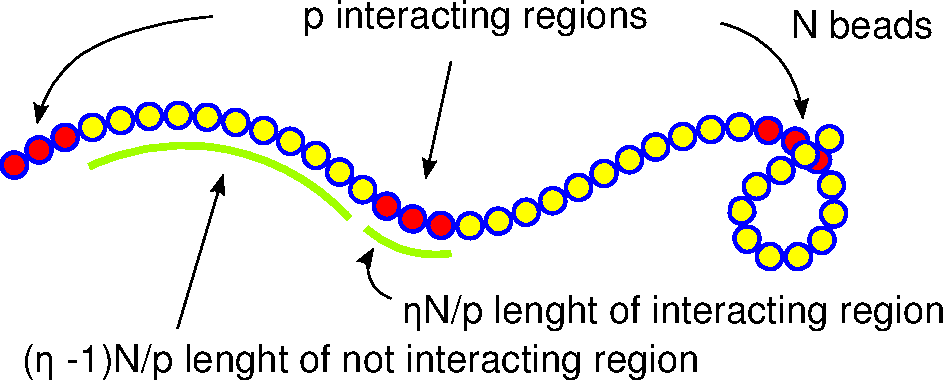
\includegraphics[width=9cm]{local_unif_config}\\
\caption{The parameters $\eta$ and $p$ define for fixed $N$ univocally
  a configuration of equispaced locally interacting regions along the
  polymer chain.}
\label{fig:locuniexpl}
\end{figure}
Those rules could be relaxed by introducing stochasticities or
information from experiments but in the following paragraph we are
going to stick to the minimal rules in order to get more insight on
the general behaviour of the system before approaching more complex
cases. We can think of this exercise as a form of mean field
approach.

As explained in section \ref{sec:themodel}, the beads belonging to the
two regions interact with each other with two different energy
parameters: $\epsilon_u$ is the uniform interaction which define an
attraction between each bead with any other and $\epsilon_l$ is the
localized interaction which belongs only to the \hns binding regions.

\subsection{Collapse due to localized interactions}
\label{loccollapse}

The first question we can ask is wherever the localized interaction
alone can induce a polymer collapse and at which values of
$\epsilon_l$ it would happen. We know that in the limit for $\eta \to
1$ the localized interactions would behave as the uniform so a
$\theta$ transition is to be expected in that limit.

Since in realistic configurations $\eta$ will be a small fraction of
the chromosome, a collapse of the volume occupied by the chain is to
be expected at growing values of $\epsilon_l$ (in comparison to
$\theta$) for smaller $\eta$, this expectation is confirmed by the
results of the simulation (see Fig. \ref{fig:locunicoll}).
\begin{figure}[h!]
\centering
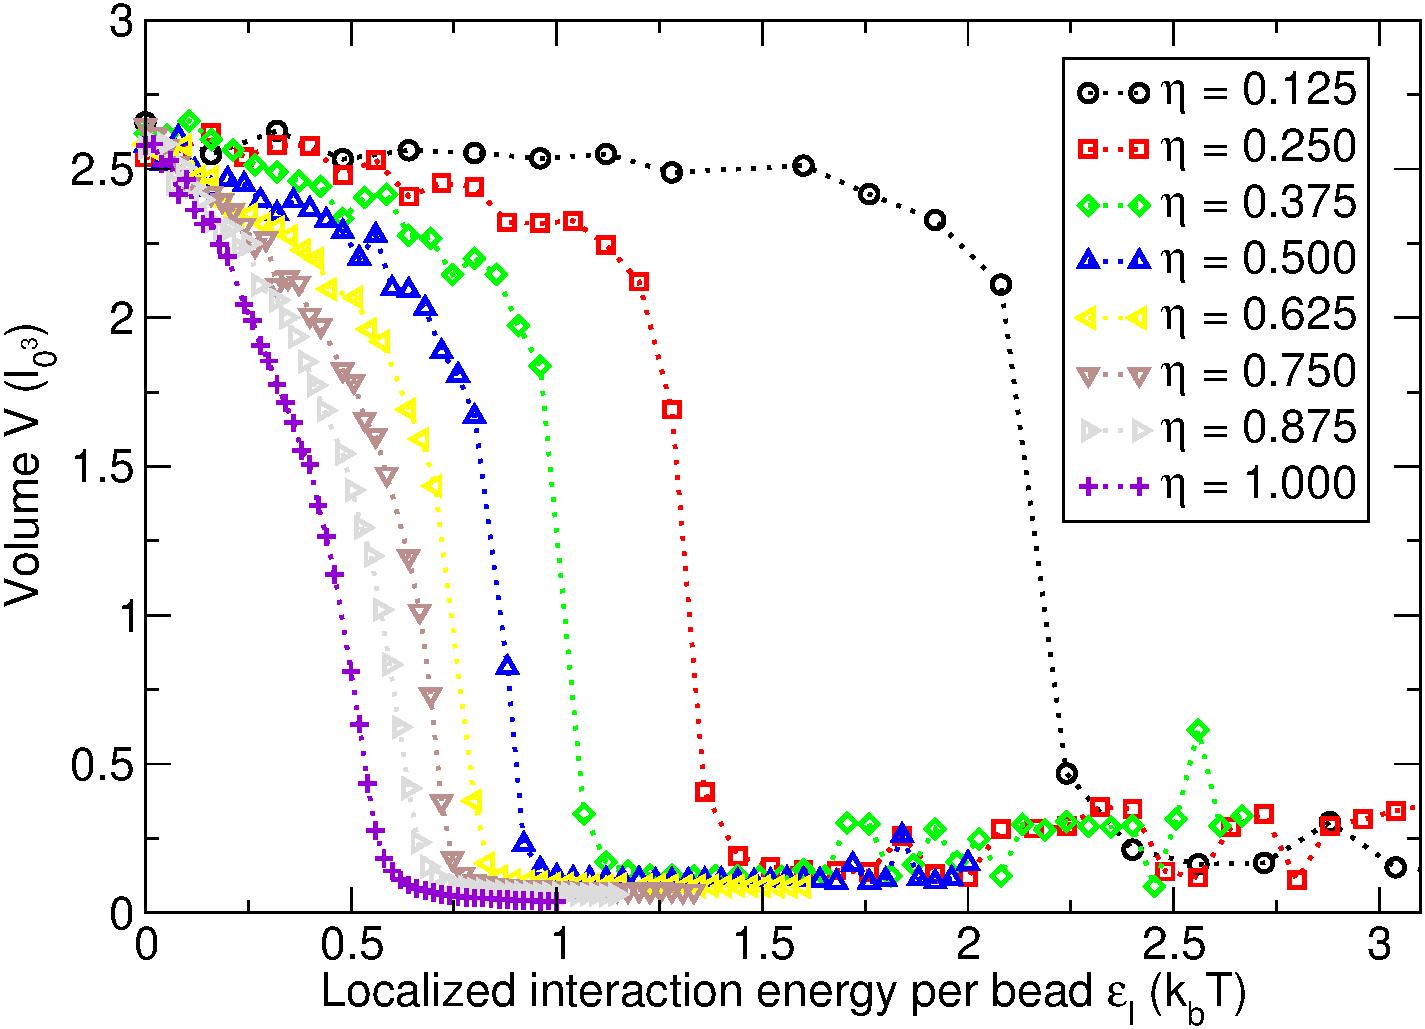
\includegraphics[width=9cm]{local_unif_collapse}\\
\caption{Collapsed of polymer as a function of local interaction energy
  $\epsilon_l$. The collapse is shown for different locally
  interaction proportion per chain $\eta$. Other parameters are set to
$(N = 256, \Sigma = 0.043, p = 16)$. The collapse of the volume of the
chain happen at higher values of $\epsilon_l$ for smaller $\eta$.}
\label{fig:locunicoll}
\end{figure}

We recall that the transition energy is fixed 
by the second virial coefficient going to zero in forumla
\ref{eq:floryent}. In the same way we write a free energy term for the
block-interactions between the $p$ identical blocks along the chain
comprising one locally interacting and one non locally interacting
region:
\begin{equation}
  F_{local} = k_b T p \left( \frac{p - 1}{2} \frac{v_{local}}{V}
  \right), \quad \mathrm{where} \quad
  v_{local} =  \left(b - \frac{a}{k_b T}\right)
\label{eq:frlocal}
\end{equation}
In order to do so we need to extimate the contributions to the
repulsive part $b$ and the attractive part $a$ to the effective
exclusion volume.

The contribution to the attractive $a$ part is given by the uniform
and localized interaction of one region with the other, $a = a_{uni} +
a_{loc}$. The uniform attraction for is between every couple of
locally interacting regions and the non locally interacting region
which sorround it, thus:
\begin{equation}
  a_{uni} = \frac{N}{p} \frac{4}{3} \pi \epsilon_u (\alpha^3 -
  \sigma^3);
\end{equation}
The local attraction instead is only between the locally interacting
regions, thus:
\begin{equation}
  a_{loc} =  \frac{N \eta}{p} \frac{4}{3} \pi \epsilon_l (\alpha^3 -
  \sigma^3). 
\end{equation}
The contribution to the repulsive $b$ part is given by the sum of the
hard core repulsion and the entropy cost of closing the loop between
two locally interacting regions, $b = b_{hc} + b_{loop}$. The hard
core repulsion can be extimated as:
\begin{equation}
  b_{hc} = \frac{N}{p} \frac{4}{3} \pi \sigma^3;
\end{equation}
while the looping entropy can be extimated at the zeroth order by
assuming the non locally interacting chains to be free, we know the
probability distribution function for the free chain from
eq. \ref{eq:probideal}, we can extimate the partition function
determined by the closing of all $p - 1$ possible loops as following:
\begin{equation}
\begin{array}{r l}
  \mathbb{Z}_{loop}(p, \eta) &=
      \left(1 - \int_{|\vec r| < \alpha} d \vec r\ p_{gN}(\vec r)
      \right)^{p-1} \quad \mathrm{with} \quad g = \frac{1 - \eta}{p}
 % = \left( 1 -
 %    \left( \frac{3}{2 \pi} \right)^{3/2}\frac{1}{V} \int_{|\vec r| <
 %      \alpha} d \vec r\ 4 \pi r^2 
 %    \exp \left( -\frac{3}{2} \frac{r^2}{V^{2/3}}\right)
 % \right)^{p-1}
\\ &=
\left(
  1 - \sqrt{\frac{6}{\pi}}\frac{\alpha}{l_0 g^{1/3}}
  e^{-\frac{3\alpha^2}{2 g^{2/3} {l_0}^2}} +
  \mathrm{Erf}\left( \sqrt{\frac{3}{2}} \frac{\alpha}{l_0
      g^{1/3}}\right) \right)^{p-1}
\\ &= \left(1 - \Xi(p, \eta)
\right)^{p-1},
\end{array}
\end{equation}
to notice that the loop partition function goes to $0$ for $\eta \to
1$ as it is expected.
The Helmholtz free energy of collapse due to this term is thus equal
to:
\begin{equation}
  F_{loop} = -k_bT (p - 1) \log \left[1 - \Xi(p, \eta) \right]
\end{equation}
taking the first order expansion of the logarithm and comparing with
eq. \ref{eq:frlocal}, putting at the transition $V = {l_0}^3$, we can
extimate an effective interaction term: 
\begin{equation}
b_{loop} = {l_0}^3\ \Xi(p, \eta)
\end{equation}

We can thus extract the energy at which the effective volume is null
by summing the four term end comparing to zero $b - a/k_bT = 0$: 
\begin{equation}
\left. \epsilon_l \right|_{v = 0} = 
\frac{\Theta_{loc} - \epsilon_u}{\eta}; \qquad
\Theta_{loc} = \Theta \left( 1 + \frac{3}{4\pi} \frac{{l_0}^3}{\Sigma} p\
  \Xi(p, \eta) \right).
\label{eq:loccrituno}
\end{equation}
This equation for the transition energy behaves as expected
for $\eta \to 1$ and $\epsilon_u \to 0$, because $\Theta_{loc} \to
\Theta$ and the polymer collapse exactly at the $\Theta$ transition;
however, as $\eta$ decrease, 
it requires an higher attractive energy $\epsilon_l$ for the
transition to happen; in the limit of small $\eta$, we can take the
first order of the expansion of
$\Xi(p, \eta)$ for the parameter $\frac{(1 - \eta)N}{p} \gg 1$:
\begin{equation}
  \Xi(p, \eta) \simeq \sqrt{\frac{6}{\pi}} \frac{\alpha^3}{{l_0}^3}
  \frac{p}{1 - \eta} = \sqrt{\frac{6}{\pi}} \frac{A_l}{{l_0}^3(1 - \eta)}.
\end{equation}
where $A_l = \alpha^3 p$ is the renormalized localized interaction
volume, the corrispettive in the uniform case was $A = \alpha^3 N$;
Also ${l_0}^3(1 - \eta)$ is a physical parameter and correspond to the
total volume occupied by the portion of the chain which is not locally
interacting at the $\Theta$ transition, the corrispettive in the
uniform case would have been ${l_0}^3$.

The dependence of the transition point can thus be approximated by the
following formula:
\begin{equation}
\left. \epsilon_l \right|_{v = 0} (\eta) 
\underset{\eta^{-1} \gg 1}{\simeq} - \frac{\epsilon_u}{\eta} + 
\frac{1 + C p}{\eta} \Theta
\label{eq:loccritsec}
\end{equation}
where $C$ is a constant that depend on other variables of the
simulation. We thus predict that,
\begin{itemize}
\item
the transition energy is equal to $\Theta$ indipendently of $p$ for
$\eta \to 1$.
\item
the transition energy is a linear function of $\eta^{-1}$ for small
$\eta$; at fixed $\eta$, the transition energy increase with an
increase of the number of interacting regions $p$.
\end{itemize}
Results of simulation confirm those two predictions (see
Fig. \ref{fig:locunicrit}). Also those results can be compared
qualitatively with the SBS (strings and binders switch)
model\cite{Barbieri2012} if we consider the proportion of interacting
regions $\eta$ as a growing function of the mean number of \hns
molecules in the living cell (see appendix \ref{logistic} for
details).
\begin{figure}[h!]
\centering
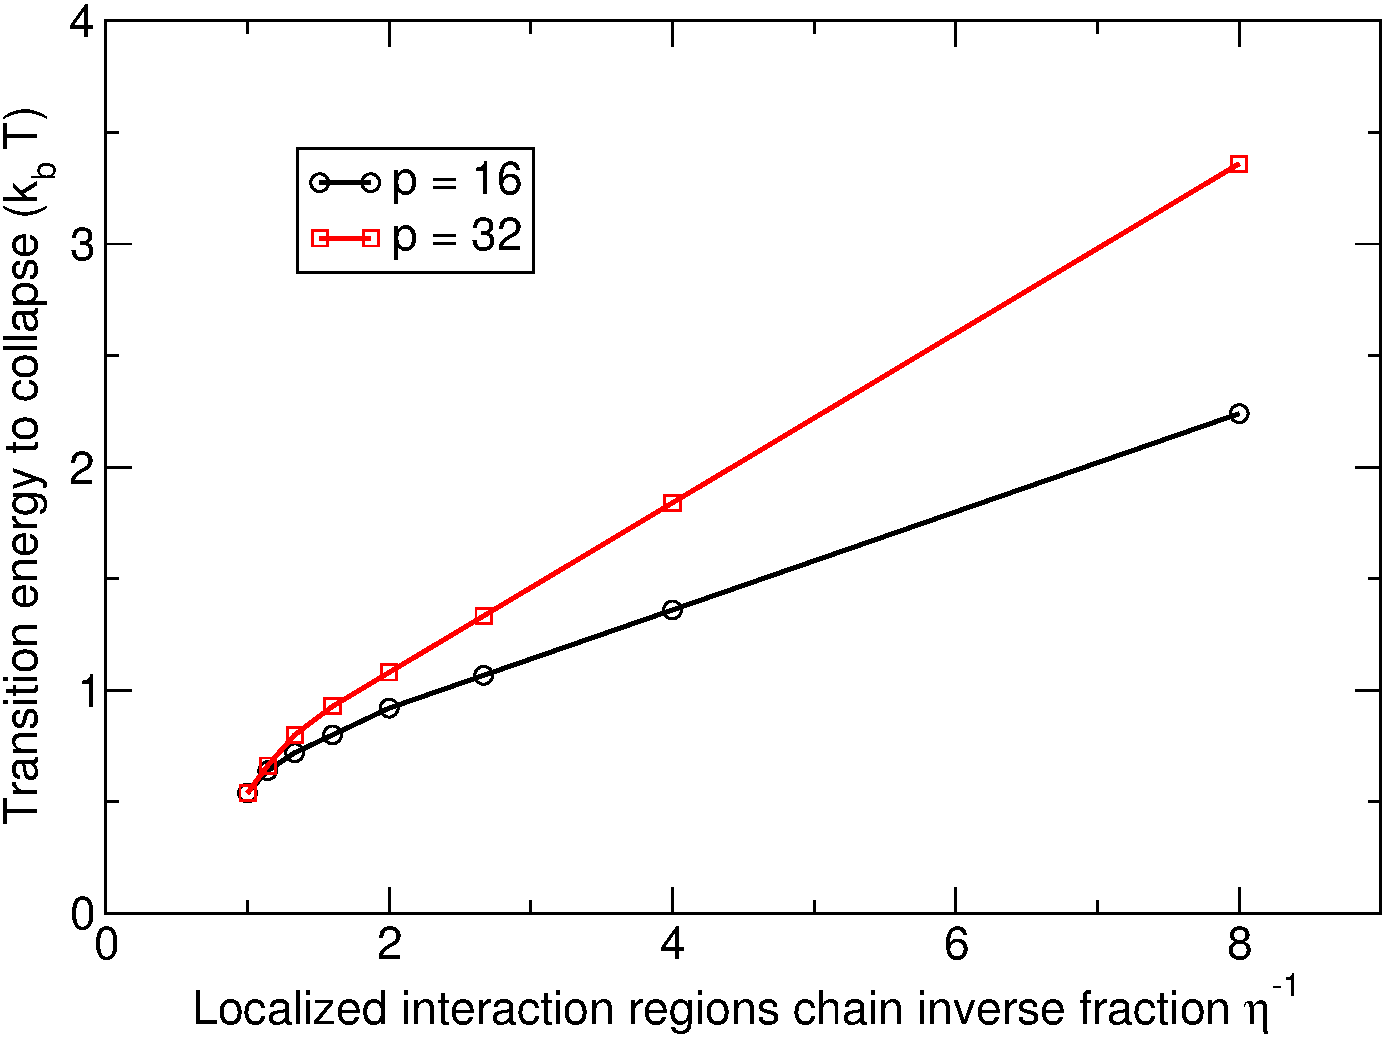
\includegraphics[width=9cm]{local_unif_critical}\\
\caption{Collapse transition energy per bead $\left. \epsilon_l
  \right|_{v = 0}$ as a function of local interaction regions fraction
  $\eta$. Measurement were taken for $p = 16$ and $p = 32$ and confirm
  the trends of equations \ref{eq:loccrituno} and
  \ref{eq:loccritsec} which predict $\left. \epsilon_l \right|_{v = 0}
  = \Theta = 0.5 k_bT$ for $\eta \to 1$, and a linear 
  dependence of the transition energy in $\eta^{-1}$ for smaller
  values of $\eta$. To note that the correction due to
  $\mathbb{Z}_{loop}$ accounts for the dependence of the transition
  energy from the $p$ parameter. Other parameters are set to $(N =
  256, \Sigma = 0.043, \epsilon_u = 0)$.}
\label{fig:locunicrit}
\end{figure}

As for the uniform interaction, we should choose a suitable set of
energy parameters which behave well under renormalization of the
number of statistical units $N$; The indipendent
extensive variables which describe the polymer energy are:
\begin{equation}
\label{eq:loccollapse}
\frac{E_1}{k_bT} = (p - 1)\left(\epsilon_l + \frac{\epsilon_u - (1 +
    C p)\Theta}{\eta}\right)
\quad \mathrm{and} \quad
\frac{E_2}{k_bT} \simeq (N - 1)(\epsilon_u - \Theta), \mathrm{\ for\ small\ }
\eta 
\end{equation}
$E_1$ represents the internal energy of the \hns
binding regions, alternatively we can call it the strong localized
beads interaction, while $E_2$ represents the internal energy of the
regions where there is no \hns binding, the soft concentrated beads
interaction and is equal to $E_u$ in the absence of localized
interactios. Those variables renormalize properly with a change of
resolution $N$ and are null at the transition point.

As in the only uniform attraction case, while the Flory-type analysis
is satisfying in the swollen case, it cannot explain the behaviour in
the collapsed phase. We can transpose some elements of the qualitative
phenomenology of the uniform collapse to this different kind of
collapse: in the cases of strong localized interaction
$(E_1 \gg 0)$ and small uniform interaction $(E_2 < 0)$, which is the
most interesting case, the size of the collapsed phase will be equal
to the portion of volume occupied by the localized beads $(V = \eta
\Sigma)$; for small globle sizes $(\eta \Sigma < \Sigma_c)$ the
transition from coil to globular phase will become
first-order-like. On the other end the effect of the localized
interactions will be big in the collapsed case due to micro-phase
segregation happening between the strongly interacting and the softly
interacting regions.

Our simulations show that the strongly interacting beads collapse in a
compact globule while the swollen regions which are softly interacting
form a branched structure on the surface. In the simpler case the
result is a structure which resemble a micelle
(see Fig. \ref{fig:micelle}). The size and the number of micelles
which are formed per polymer is not constant across the parameter space.

\subsection{Micelle size and properties}
\begin{figure}[h!]
\centering
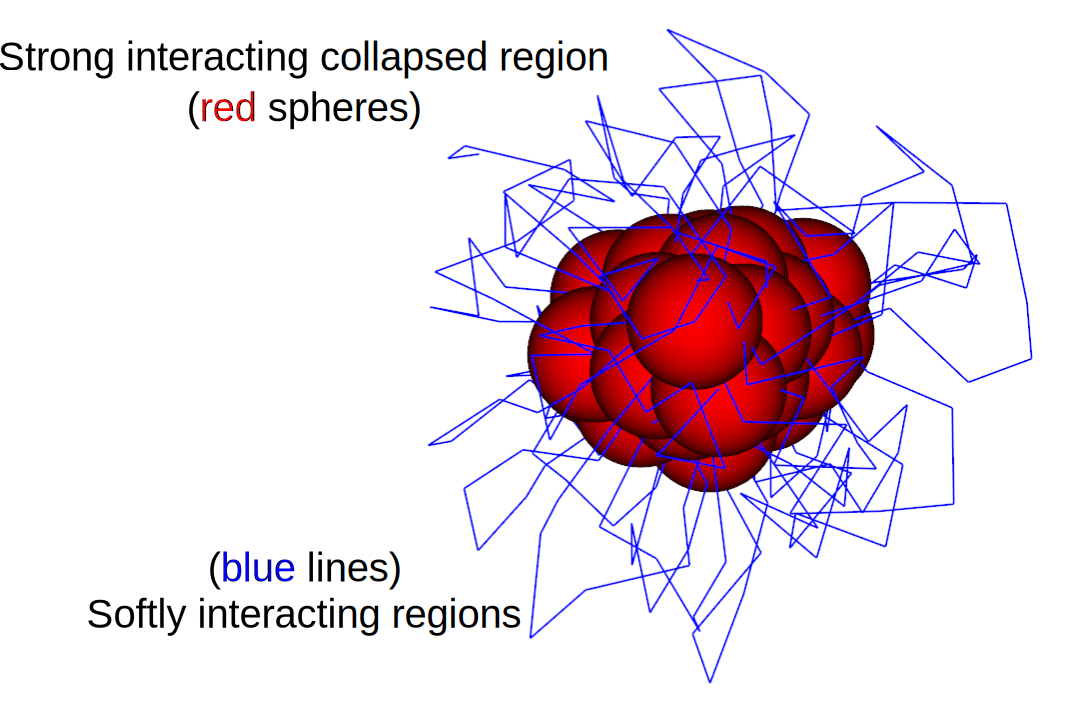
\includegraphics[width=12cm]{micelle}
\caption{Strongly interacting and softly interacting regions can
  self-assemble to form a structure that reflect a polymeric micelle.}
\label{fig:micelle}
\end{figure}

The formation of a micelle is an evidence of self-assembly of the
bacterial nucleoid structure. The theory for explaining the size and
the stability of this structure can be studied by
implementing the mothodology developed for membrane micelles in
the book of Israelachvili \cite{israelachvili2011}. The theory of
membrane micelles predict that there is a typical micelle size in
function of the microscopical parameters which is set by the
equilibrium between the repulsion between the hydrophilic heads on the
surface and the attraction of the hydrophobic tails. If the
concentration of surfactant molecules is high enough, due to this
typical micelle size, multiple micelles are produced in solution with
a size distribution which is peaked around the typical micelle size
till the number of isolated surfactant molecules goes to a small
quantity (called the critical micelle concentration).

In our simulations micelles are formed in the conditions where we set
a strong localized attractive interaction $(E_1 \gg 0)$, which keeps
the core of the micelle in a collapsed state comparable to the
hydrophobic portion of surfactant micelles, and a negative uniform
interaction $(E_2 < 0)$ which in turns creates a corona of swollen
chain around the core as in Fig. \ref{fig:micelle}.

Since the localized attractive beads and the other beads phase
segregate in a swollen corona and a collapsed core, which are
sub-structures with a big difference in the dynamics, we can
use an adiabatic approximation and write the free energy of the
a micelle formed by $n$ localized interaction regions as a sum of the
free energy of the core and that of the corona:
\begin{equation}
F_{micelle}(n, V, E_1, E_2) = F_{core}(n, E_1) + F_{corona}(n, V, E_2),
\end{equation}
with $p$ and $\eta$ fixed, also, for stable micelles we can ignore the
fluctuations in the volume $V_{core}=n \eta \Sigma / p$ of the core
which are negligible in comparison to the space fluctuations of the
swollen corona.

The size and the number of micelles formed in the
single polymer is not constant across the parameter space. We can
expect this fenomenology due to the physical analogy of our sistem to
a surfactant colloidal solution confined by the link chain. The volume
of a single micelle is going to increase with the decrease of the
parameter $E_2$ since it correspond to an increase of the effective
volume of the beads and thus to a swelling of the corona around the
globule; correspondingly, it is expectable a monotonical increase of
$F_{corona}$ as a function of the decrease of the $E_2$ parameter. At
some point $F_{corona}$ is going to outweight $F_{core}$ in the
micelle free energy because $F_{core}$ is expected to stay
approximately constant as a function of $E_2$. The question is if there
is a critical corona energy $E_2$ under which a polymer with a single
micelle undergoes fission and the stable polymer configuration shows
states with two, or multiple micelle.

In order to answer this question we simulated the polymer with fixed
$p$, $\eta$ and $E_1$ starting from a initial configuration which
correspond to a single micelle per polymer
(Fig. \ref{fig:micelle}), lowering the uniform interaction parameter
$E_2$ in order to find a transition to a multiple micelle
configuration. The initial configuration was fixed by running the
system with the corona at the theta transition $E_2 =0$, in
this conditions the free energy of the corona is purely enthropic and
thus there are no elements which would suggest a free energy advantage
of the multiple micelle scenario over the single micelle one.

While we expect the transition between a single micelle to a two micelle
scenario to not change the volume of the fluctuations of the polymer
by a great amount, we do expect the breaking of the rotational
simmetry around the three space dimensions. This simmetry breaking is
not something unusual in such transition and is present also in the
coil-globule transition. We expect this breaking because fluctuation
of the volume occupied by the polyme along the vector which connects
the two cores would be bigger than the fluctuation around the other
two axis of simmetry of the two cores taken individually (see
Fig. \ref{fig:simmbr}).

\begin{figure}[h!]
\centering
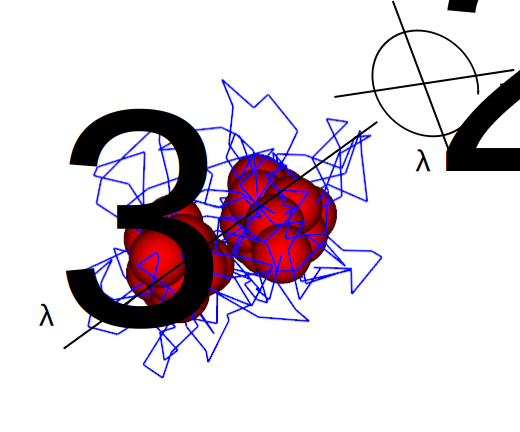
\includegraphics[width=8cm]{simmbr}
\caption{The volume occupied by the polyme along the vector which connects
the two cores would be bigger than the fluctuation around the other
two axis of simmetry of the two cores taken individually.}
\label{fig:simmbr}
\end{figure}

It is possible to measure this effect by taking the mean of the
ratio of the first and the third eigenvalue of the inertia matrix of
single realization along the montecarlo time.
\begin{equation}
\Gamma = \left\langle \frac{\lambda_1}{\lambda_3} \right\rangle \quad
\mathrm{where} \quad \det(I - \lambda_i) = 0 \quad \mathrm{and}\ I\
\mathrm{is\ the\ inertia\ matrix\ of\ single\ configuration}
\end{equation}
we measured this quantity in simulations as well as the volume
as a function of the corona interaction energy $E_2$, we were able to
show, for a sufficient number of statistical units $N$, the micelle
binary fission under a critical corona energy $E_2^{crit}$ (see
Fig. \ref{fig:inertion} and Fig. \ref{fig:unif8contact}).

\begin{figure}[h!]
\centering
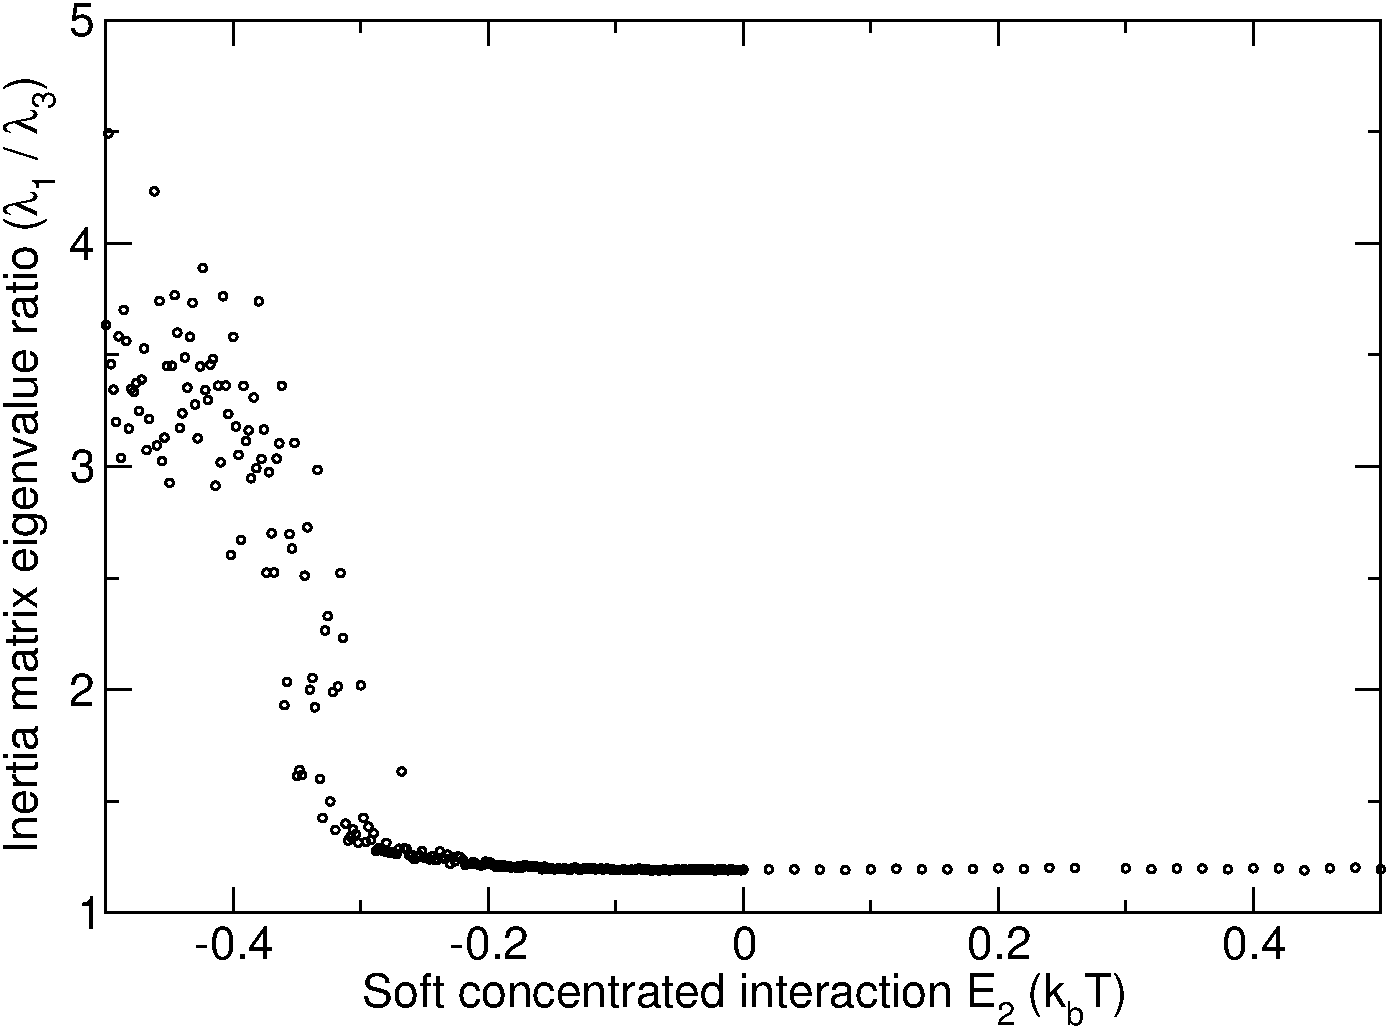
\includegraphics[width=9cm]{inert_loc_eq}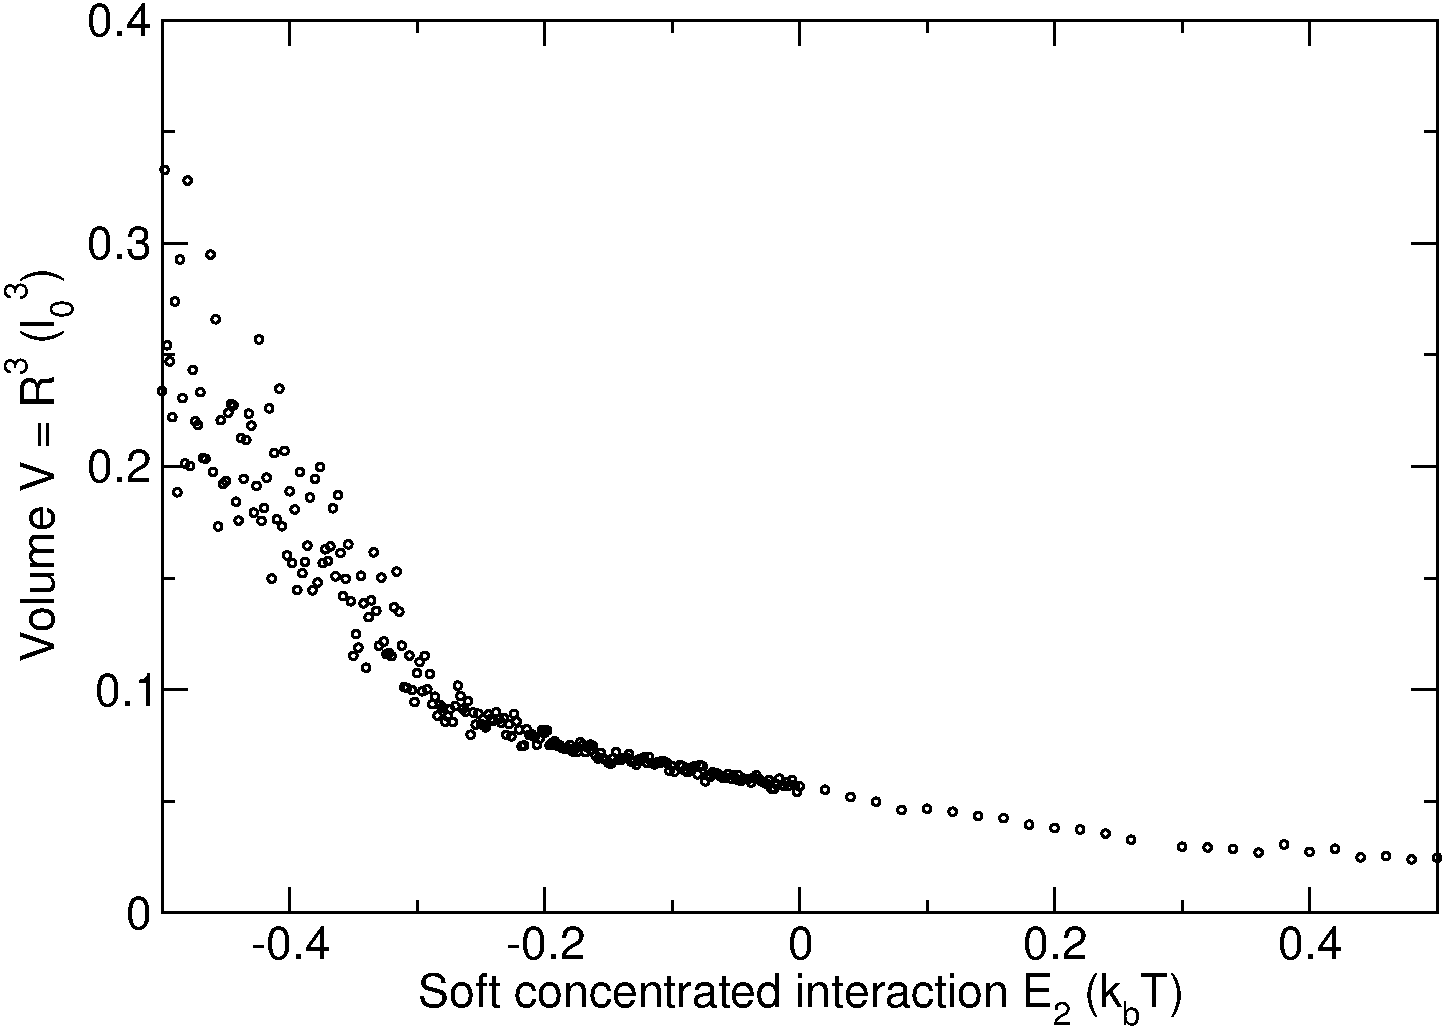
\includegraphics[width=9cm]{r_loc_eq.pdf}\\
\caption{Left: mean ratio between the first and the third eigenvalue
  of the inertia matrix ($\Gamma$) over single realizations along the
  montecarlo time as a function of the corona energy $E_2$. Right:
  Volume occupied by the fluctuations of the end-to-end distance in
  function of corona energy $E_2$. The plot show a phase transition at
  the energies for which the single micelle fission in two
  micelles. The other parameters of the simulation are set to:
  $(\epsilon_u + \epsilon_l = 3.4, \eta = 0.125, p = 32, N = 256$,
  $\Sigma = 0.042 \cdot {l_0}^3)$.
}
\label{fig:inertion}
\end{figure}

\begin{figure}[h!]
\centering
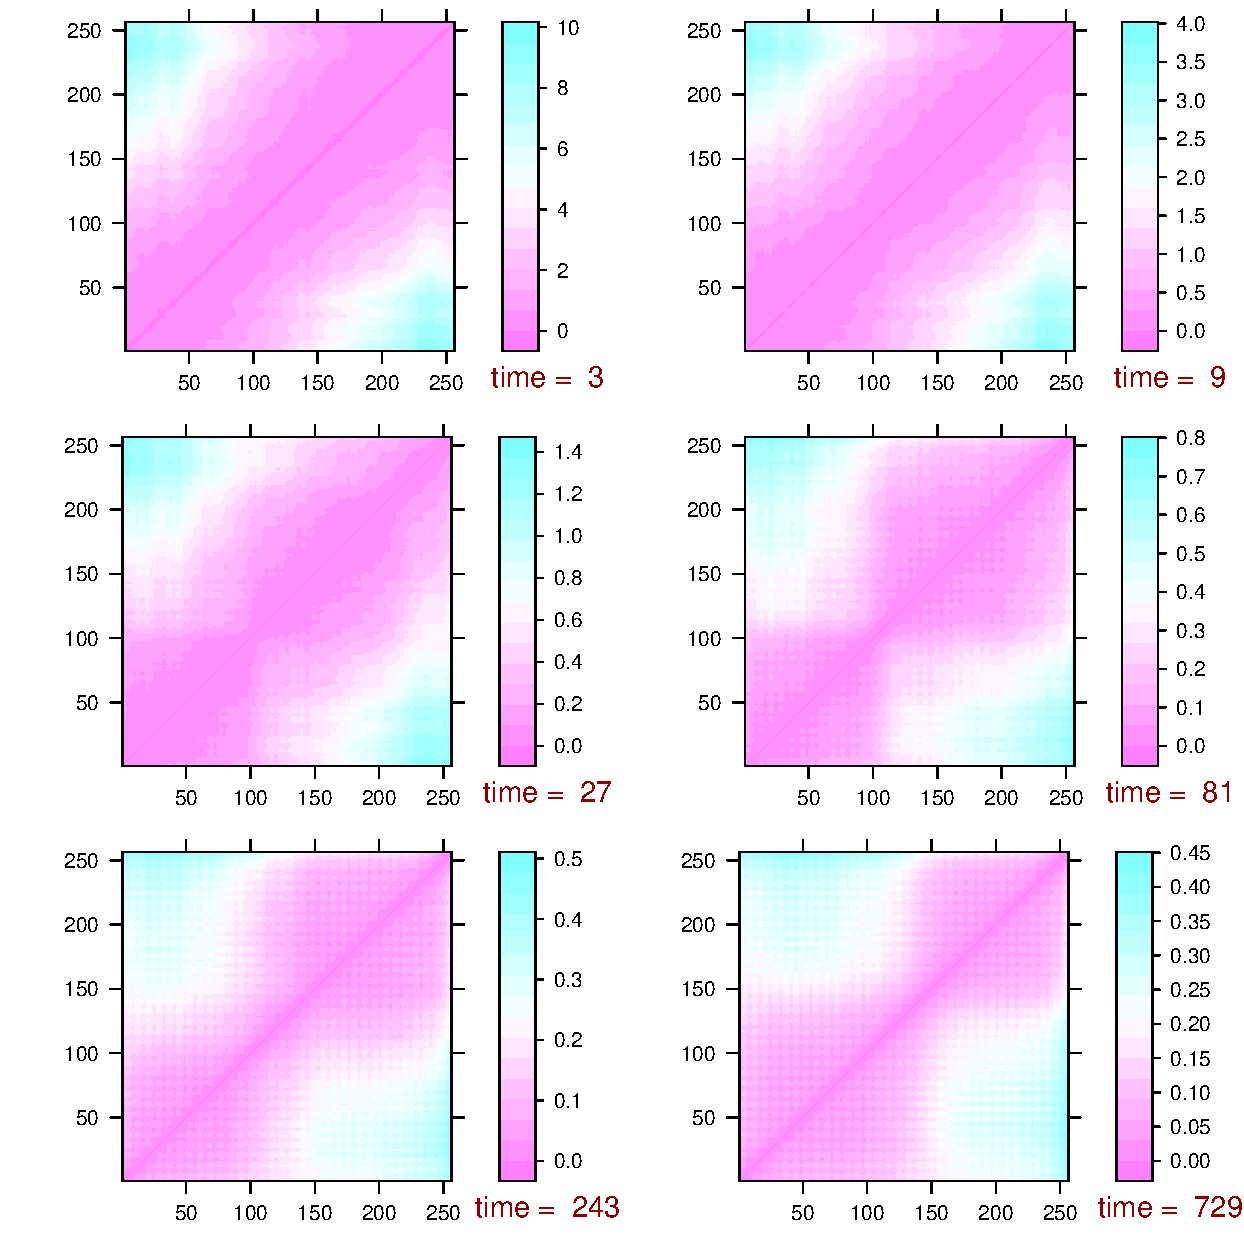
\includegraphics[width=11.5cm]{unif8contact}
\caption{Contact matrix for a polimer with localized interactions in
  function of time. This figure show the collapse of the polymer in
  two different micelles. The
  matrix are plotted for ineteraction energies and localized
  interaction configuration $(\epsilon_u = 0,
  \epsilon_l = 3.4, \eta = 0.125, p = 32)$. The
  polymer have the following parameters: $N = 256$, $\Sigma = 0.042
  \cdot {l_0}^3$. The simulations are started with
  initial condition of the swollen coil and the mean contact matrix
  is measured over $6$ different time ranges.} 
\label{fig:unif8contact}
\end{figure}

A binary fission of the micelle is to be expected given the condition of
$F_{micelle}(n, E_1, E_2) > 2 \cdot F_{micelle}(n/2, E_1, E_2)$. We
can generalize and write the free energy of $q$ micelles, trascuting
any interaction term:
\begin{equation}
F_{micelles}(n, q, V, E_2) = q F_{micelle}(n/q, V, E_2)
\label{eq:fission}
\end{equation}

The free energy of the core can be extimated as follows:
the energy carried by the beads which are deep inside the cores
carry a fixed energy indipendent of the number of micelles because
they at most interact with a fixed number of core beads, proportional
to the ratio $(A - \Sigma)/\Sigma$; the beads which are instead on the
surface of the core interact only on the side which is in contact with
other core beads thus they will carry only a fraction of the energy
carried by the beads deep inside the core. The
energy difference between the surface and the central beads create a
surface tension of the globule. The surface tension is the force which
keeps spherical shape of the globule and avoid the splitting of it in
order to minimize the core surface. The energy is can be written
as\cite{israelachvili2011}:
\begin{equation}
F_{core} = \gamma a,
\end{equation}
where $\gamma$ is the a function of $E_1$ and $a$ is the surface area
of the core. Since we know that the volume of the core made by $n$
localized interacting beads, for $E_1 \gg 0$ is $V_{core} \simeq 
\eta \Sigma n / p$, we can extimate $F_{core}(n, E_1) = \gamma(E_1)\cdot(
\eta \Sigma n / p)^{2/3}$. The free energy carried by $q$ cores is:
\begin{equation}
F_{cores}(n, q, E_1) = q\cdot F_{core}(n/q, E_1) =
q^{1/3} F_{core}(n, E_1)
\end{equation}
which increase by increasing the blob number $q$.

Without approaching the problem of the eximation of the free energy of
the corona as a function of the number of interacting regions $n$, we
can guess already that if the free energy is a power law this
parameter:
\begin{equation}
F_{corona}(n, V, E_2) = \nu(E_2, V) n^{\rho}
\label{eq:coronapow}
\end{equation}
then the corona free energy carried by $q$ micelles is also a power
law of the blob number $q$:
\begin{equation}
F_{coronas}(n, q, V, E_2) = q^{1 - \rho} F_{corona}(n, V, E_2)
\end{equation}
with exponent $1 - \rho$. In order to have an equilibrium number of
micelles which is different from $1$ it thus suffice to have the
exponent $\rho > 1$.

We can extimate the form of eq. \ref{eq:coronapow} by analogy with the
free energy of the star polymer. Daoud and Cotton studied the density
shape of the star polymer using a blob representation\cite{Daoud1982},
they extimate the size of the thermal blob as a function of the distance
$r$ from the star polymer center to be $\xi \sim r f^{1/2}$  where $f$
is the number of branches. They also suppose that considering the volume
of between the spheres of radius $r$ and $r + \xi$ the whole shell
contains $f$ blobs, one for each branch. Thus the total number of
blobs per star polymers should scale as $n_{blobs} \sim f \xi^{-1}
\sim f^{3/2}$. If, as an analogy, we compare the corona of a micelle
to a star polymer with $2 n$ branches, we can extimate using the blob
ansatz ($F \sim k_b T$ per number of blobs) the exponent $\rho =
3/2$. Using this extimation we can write:
\begin{equation}
F_{micelles} = q^{1/3} F_{core}(n, E_1) + 
\frac{1}{q^{1/2}}F_{corona}(n, V, E_2)
\end{equation}
The number of micelles which minimises the energy is thus equal to:
\begin{equation}
  q = \left( \frac{3}{2} 
    \frac{F_{corona}(n, V, E_2)}{F_{core}(n, E_1)} \right)^{6/5}
\end{equation}
If we replace $n$ by $p$, we can extimate using this formula the
number of micelles per chain: by increasing the weight of $F_{corona}$
to $F_{core}$, for instance by reducing the negative corona energy
$E_2$ we increase the stability of the splitted micelle $q > 1$ case
respect to the single micelle.

The behaviour of polymeric micelles is very similar to the case of
polysoaps. Polysoaps are hydrophilic polymers which
incorporate amphiphilic monomers, the hydrophilic part of the polysoap
is swollen while the amphiphilic part is collapsed due to the
interaction with the solvent by definition; this situation is similar
to the collapsed phase of our model with strong localized interaction
and small uniform interaction. It has been shown that also polysoap
forms micelles of different size and number, also the interactions
their interactions of the micelles between each other give place to
complex ternary structures\cite{Borisov1996,Borisov1997}.

\begin{figure}[h!]
\centering
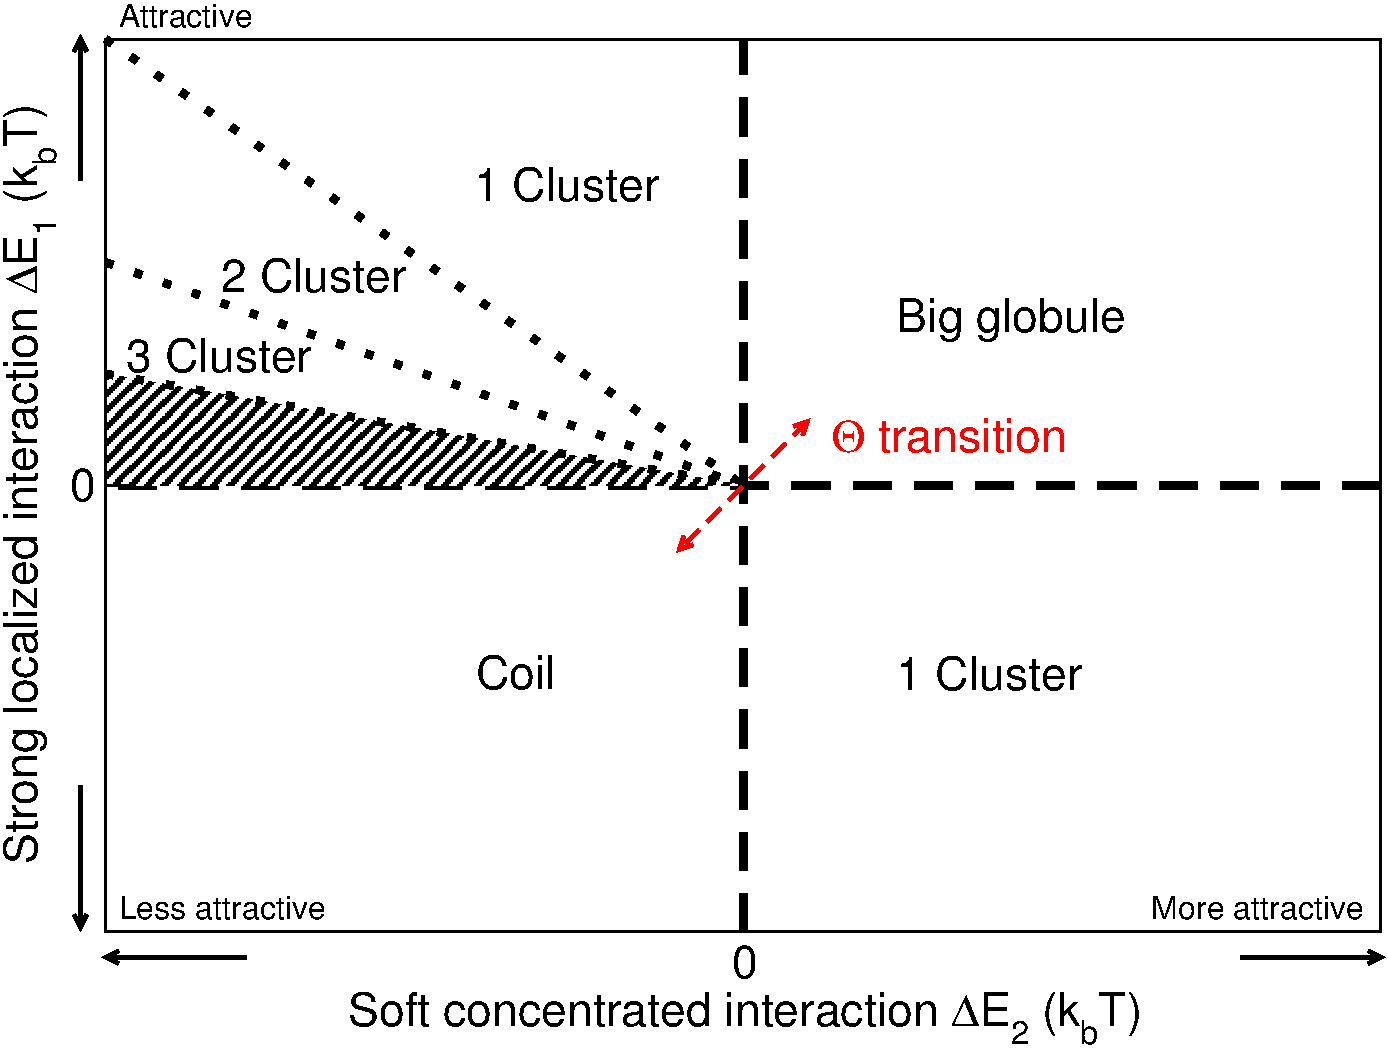
\includegraphics[width=8.5cm]{local_phases}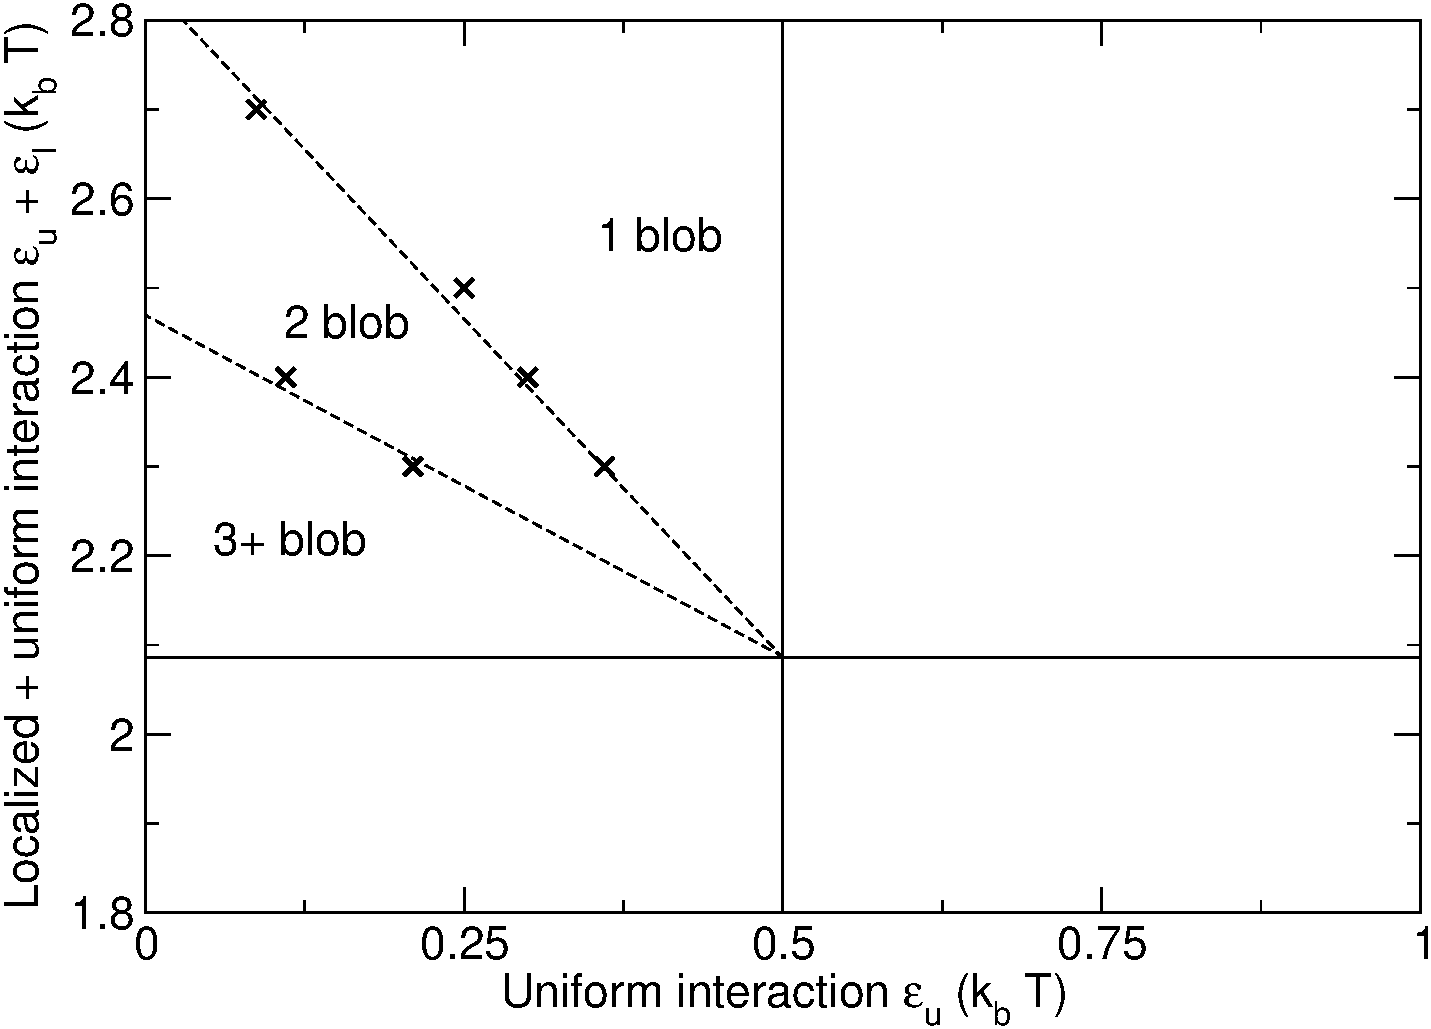
\includegraphics[width=8.5cm]{zexpclust}\\
\caption{Theoretical phase diagram of micelle formation and results
  from simulations (hand made/totally unreliable). Simulation
  parameters are $(N=256, \Sigma=0.043, \eta=0.125, p=32)$.
} 
\label{fig:locphases}
\end{figure}

% \subsection{Dynamics of micelle interactions and micellar-polymer
%   conformations}

\FloatBarrier

\section{Contact matrices and contact probabilities from HiC experiments} 

\subsection{Typical contact matrices in different polymer phases from
            simulations}

\begin{appendices}
\section{Binding profiles as a function of concentration and specificity}
\label{logistic}
The section \ref{loccollapse} describe the collapse of the polymer in
function of the localized interactions. We learned that the transition
energy is equal to $\Theta$ in the limit for $\eta \to 1$ and that it
increase with $\eta^{-1}$ and $p$. While $\eta$ and $p$ are very
convenient parameters for the calculation purpouse, we would like in
this section to address the problem of extimating the collapse energy
of etheropolimer in function of the \hns concentration which is more
close to the possible experimental verifications of the model.

In this simplified model we will consider the lenght of \hns binding
regions as fixed to $\eta / p$. In order to extract the transition
energy per bead $\left. \epsilon_l \right|_{v = 0}$  (see
eq. \ref{eq:loccritsec}) in function of \hns concentration we will
thus simulate the collapse at fixed $p$ with $\eta / p$ fixed, then we
will apply a trasformation which redefines the axes 
$(p, \epsilon_l) \to (c(p,\epsilon_l), \epsilon_l)$ with $c(p,
\epsilon_l)$ concentration of \hns molecules that will be
appropriately defined in the following paragraphs.

The binding probability of a transcription factor to specific sites
follows in the most simple case the logistic equation
\cite{Ackers1982,Bintu2005}. We will transcure in this work the
experimental evidence that \hns binding regions are a results
of an interplay between specific binding and
oligomerization\cite{Gordon2011, Stella2005} because this effect are
difficult to quantify. If, in general, we define with the letters $E$
the binding of a protein and $S$ the protein by itself, we can write
the equation for the chemical binding of the protein with it's binding
sites:
\begin{equation}
S + E \xrightleftharpoons[k^{-}]{k^{+}} ES
\end{equation}
This, with the law of concentration of the total number of binding
sites $[E_0] = [E] + [ES]$ let us wite an equation for the
concentration at the steady state:
\begin{equation}
\frac{[ES]}{[E_0]} = \frac{[S]}{\frac{k^{-}}{k^{+}} + [S]}.
\end{equation}

Finally we can use Arrhenius law to extimate the value of
$k^{-}/k^{+}$: and obtain the probability of a binding site to be
bound in function of the concentration of binding molecules $c \equiv
[S]$:
\begin{equation}
\mathscr{P}_{\mathrm{bound}} = \frac{c}{e^{-\frac{E}{k_b T}} + c},
\end{equation}
where $E$ is the energy per binding site (see $E_1$ in 
eq. \ref{eq:loccollapse}): $\frac{E}{k_bT} \sim \epsilon_l$ for
$\epsilon_u$ and $\Theta$ small. And $c$ can be expressed in protein
units per base pair.

On the \ecoli chromosome there are multiple \hns binding sites. The
number $N$ of binding sites per chromosome has been extimated in
\cite{Kahramanoglou2011} to be respectively $458$ in middle
exponential phase and $537$ in stationary phase. We can write the
number of occupied \hns binding sites as:
\begin{equation}
p = N \mathscr{P}_{\mathrm{bound}} = 
    N \frac{c}{e^{-\epsilon_l} + c},
\end{equation}
inverting we finally find the equation for $c(p,
\epsilon_l)$:
\begin{equation}
c(p, \epsilon_l) = \frac{p}{N-p} \exp (\epsilon_l).
\label{eq:ci}
\end{equation}
Thus we now we have a tool to substitute in the graphs the parameter
$p$ with the concentration $c$. The results of this substitution is a
phase diagram comparable to the one optained by Nicodemi
\cite{Barbieri2012} and an example is reported in Fig
\ref{fig:znico}. In line to the Nicodemi work, in this calculation we
are not considering the fact that multiple \hns molecules binds to
single binding sites, the fact that the different binding sites have a
size distribution and the and the cohoperativity between \hns binding.


\begin{figure}[h!]
\centering
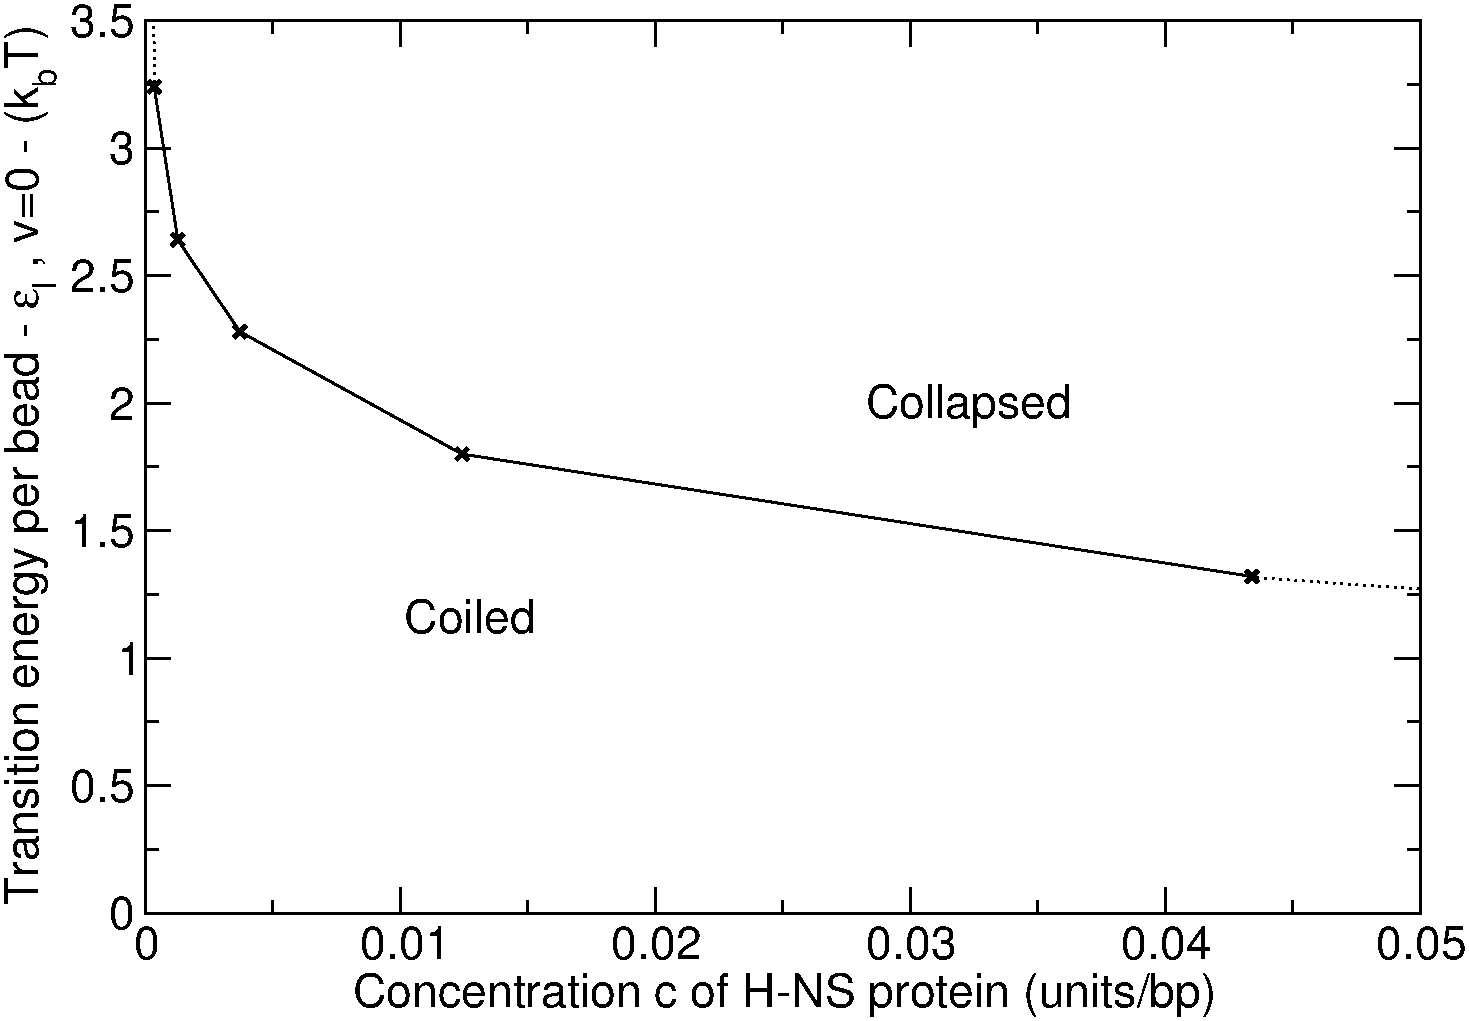
\includegraphics[width=9cm]{zNicodemi}
\caption{The simulations have been runned with parameters $N = 256$,
  $\Sigma = 0.043$, $\eta/p = 0.250/32$ and variating $p$ in ${4, 8,
    16, 32, 64}$. The points of collapse $(p, \epsilon_l)$ have then been
  converted to cohordinates $(c, \epsilon_l)$ using the transformation
  in eq. \ref{eq:ci}.
}
\label{fig:znico}
\end{figure}

\end{appendices}

\bibliography{bd.bib}{}
\bibliographystyle{plain}

\end{document}


